% CENG 467 – Take-Home Midterm Report
% Compile with: pdflatex main.tex (run twice for references)
% Required packages: listed in \usepackage commands below

\documentclass[12pt, a4paper]{article}

% ── Packages ──────────────────────────────────────────────────────────────────
\usepackage[utf8]{inputenc}
\usepackage[T1]{fontenc}
\usepackage[english]{babel}
\usepackage[top=2.5cm, bottom=2.5cm, left=2.5cm, right=2.5cm]{geometry}
\usepackage{amsmath, amssymb}
\usepackage{graphicx}
\usepackage{subcaption}
\usepackage{booktabs}
\usepackage{multirow}
\usepackage{hyperref}
\usepackage{listings}
\usepackage{xcolor}
\usepackage{float}
\usepackage{enumitem}
\usepackage{microtype}
\usepackage{parskip}
\usepackage{natbib}

% Code listing style
\lstset{
    basicstyle=\footnotesize\ttfamily,
    breaklines=true,
    frame=single,
    numbers=left,
    numberstyle=\tiny,
    keywordstyle=\color{blue},
    commentstyle=\color{gray},
    stringstyle=\color{orange},
    language=Python,
    showstringspaces=false,
    tabsize=4,
}

% Hyperref setup
\hypersetup{
    colorlinks=true,
    linkcolor=blue,
    urlcolor=blue,
    citecolor=blue,
}

% ── Title ─────────────────────────────────────────────────────────────────────
\title{
    \Large \textbf{CENG 467 — Natural Language Understanding and Generation}\\[0.5em]
    \large Take-Home Midterm Examination Report
}
\author{
    Student Name: \textbf{Mert Güden}\\
    Student ID: \textbf{300201013}\\[0.3em]
    Department of Computer Engineering\\
    Izmir Institute of Technology\\[0.3em]
    \texttt{mertguden@std.iyte.edu.tr}
}
\date{
    Submission Date: April 30, 2026\\[0.3em]
    Repository: \url{https://github.com/Mrtuzy/CENG467-TakeHome}
}

% ── Document ──────────────────────────────────────────────────────────────────
\begin{document}

\maketitle
\thispagestyle{empty}

\begin{abstract}
This report presents the implementation and experimental analysis of five core NLP tasks:
text classification, named entity recognition, text summarization, machine translation, and
language modeling. For each task, we compare multiple modeling approaches ranging from
classical machine learning to pre-trained transformer-based models. All experiments are
fully reproducible with fixed random seeds (seed = 42), consistent dataset splits, and
documented hyperparameters. The code and notebooks are available at the repository link
above. Key findings are: pre-trained transformer models consistently outperform classical and task-specific neural baselines across all tasks — DistilBERT achieves 92.96\% accuracy versus 89.66\% for TF-IDF on sentiment classification, BERT reaches F1~=~0.909 versus 0.872 for BiLSTM-CRF on NER, and MarianMT scores BLEU~36.25 versus 26.74 for a seq2seq model on English-to-German translation. Classical approaches remain competitive when neural models are under-resourced: TF-IDF outperforms the BiLSTM on classification, and extractive methods (LexRank ROUGE-1~=~0.350) are fast and faithful alternatives to abstractive models (BART ROUGE-1~=~0.438). On language modeling (WikiText-2), once trained for the full 6-epoch budget the LSTM clearly wins (test PPL~97.00) over the small Transformer (117.32) and the Kneser-Ney trigram baseline (375.69). Overall, the results confirm a clear trade-off between the performance ceiling of pre-trained models and the efficiency and interpretability of lightweight baselines.
\end{abstract}

\newpage
\tableofcontents
\newpage

% ── Q1 ────────────────────────────────────────────────────────────────────────
\section{Question 1: Representation Learning in Text Classification}
% Q1 classification section

\subsection{Problem Formulation}
We study binary sentiment classification on movie reviews. Given a review $x$, the task is to predict a label $y \in \{0,1\}$ where $0$ denotes negative sentiment and $1$ denotes positive sentiment. The goal is to compare sparse, dense, and contextual representations under a consistent evaluation protocol.

\subsection{Dataset Description}
We use the IMDb dataset with the official train and test splits, and create a stratified 10\% validation split from the training set (seed 42). The data are balanced across classes.

\begin{table}[H]
\centering
\caption{IMDb dataset statistics.}
\begin{tabular}{lrrrr}
\toprule
\textbf{Split} & \textbf{Examples} & \textbf{Avg Len} & \textbf{Positive} & \textbf{Negative} \\
\midrule
Train & 22,500 & 233.86 & 11,250 & 11,250 \\
Validation & 2,500 & 233.17 & 1,250 & 1,250 \\
Test & 25,000 & 228.53 & 12,500 & 12,500 \\
\bottomrule
\end{tabular}
\end{table}

\subsection{Methodology}
\textbf{Preprocessing and tokenization.} We compare two tokenization strategies: (i) a classical pipeline using NLTK word tokenization with optional lowercasing and stopword removal, and (ii) the DistilBERT tokenizer for contextual modeling. For the classical pipeline, we run an ablation over four configurations (A1--A4) and pick the best validation accuracy. A truncation study shows that larger token budgets improve validation accuracy (100 tokens: 0.8444, 200 tokens: 0.8720, 400 tokens: 0.8948).

\textbf{Models.}
\begin{itemize}[leftmargin=*]
		\item \textbf{TF-IDF + Logistic Regression} (sparse): unigram and bigram TF-IDF features with linear classifier.
		\item \textbf{BiLSTM + GloVe} (dense static): word embeddings initialized with GloVe 100d, BiLSTM encoder, mean pooling, and linear output.
		\item \textbf{DistilBERT} (contextual): fine-tuned DistilBERT for sequence classification.
\end{itemize}

\subsection{Experimental Setup}
We use fixed seed 42, a stratified validation split, and evaluate once on the test set. Metrics are Accuracy and Macro-F1. Training time is recorded for each model. Confusion matrices and training curves are saved for analysis.

\subsection{Results}
\begin{table}[H]
\centering
\caption{Test set results for Q1.}
\begin{tabular}{lccc}
\toprule
\textbf{Model} & \textbf{Representation} & \textbf{Accuracy} & \textbf{Macro-F1} \\
\midrule
TF-IDF + LR & Sparse & 0.8966 & 0.8966 \\
BiLSTM + GloVe & Dense (static) & 0.8898 & 0.8898 \\
DistilBERT & Contextual & 0.9296 & 0.9296 \\
\bottomrule
\end{tabular}
\end{table}

\begin{figure}[H]
\centering
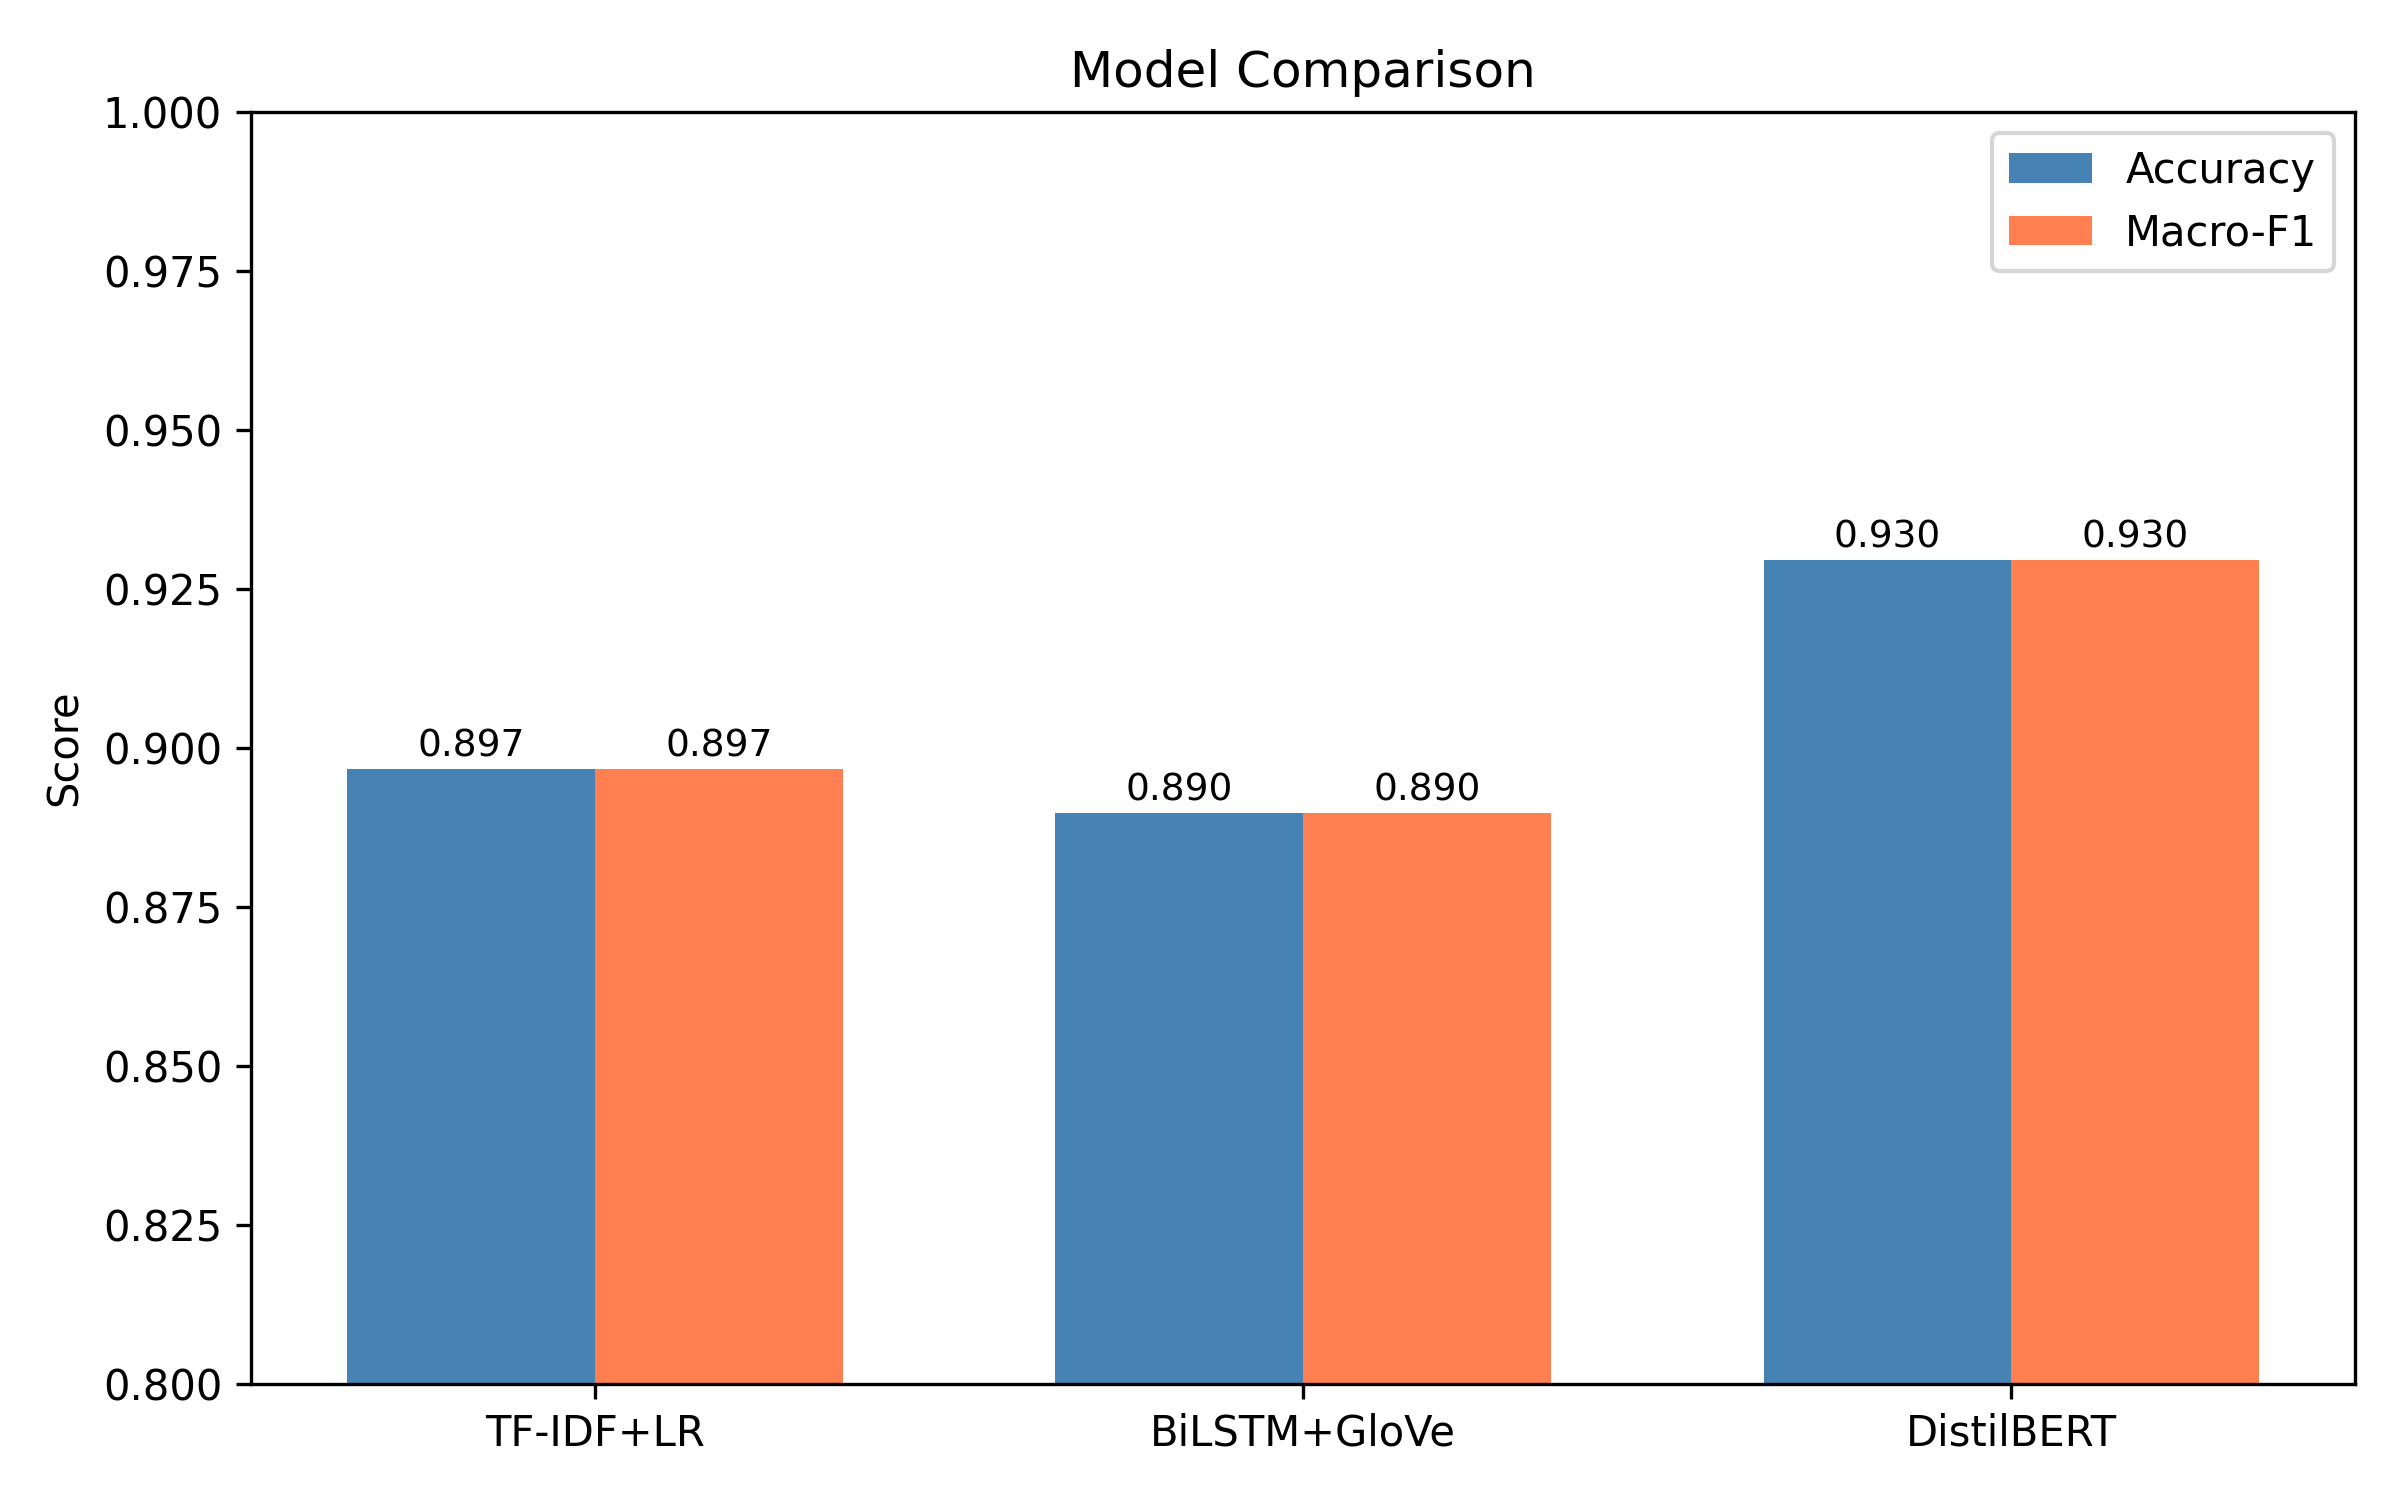
\includegraphics[width=0.78\linewidth]{../q1_classification/outputs/figures/model_comparison.png}
\caption{Accuracy and Macro-F1 comparison across models.}
\end{figure}

\begin{figure}[H]
\centering
\begin{subfigure}{0.32\linewidth}
	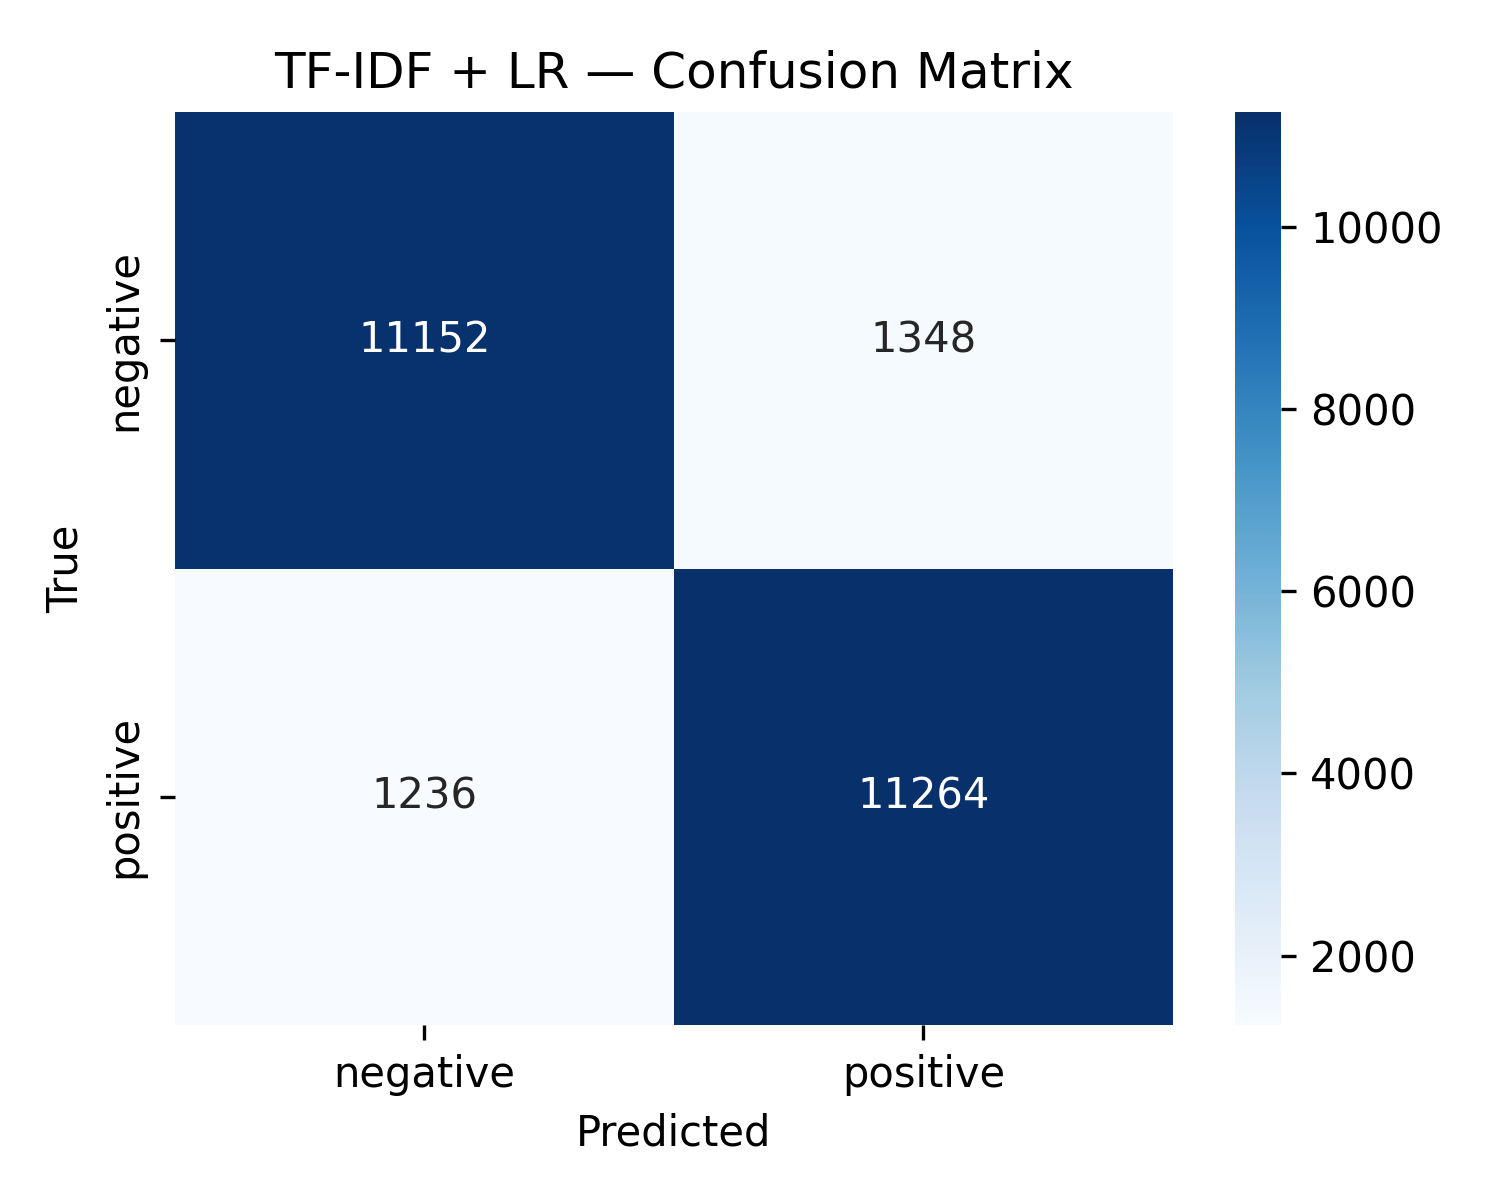
\includegraphics[width=\linewidth]{../q1_classification/outputs/figures/cm_tfidf.png}
	\caption{TF-IDF + LR}
\end{subfigure}
\begin{subfigure}{0.32\linewidth}
	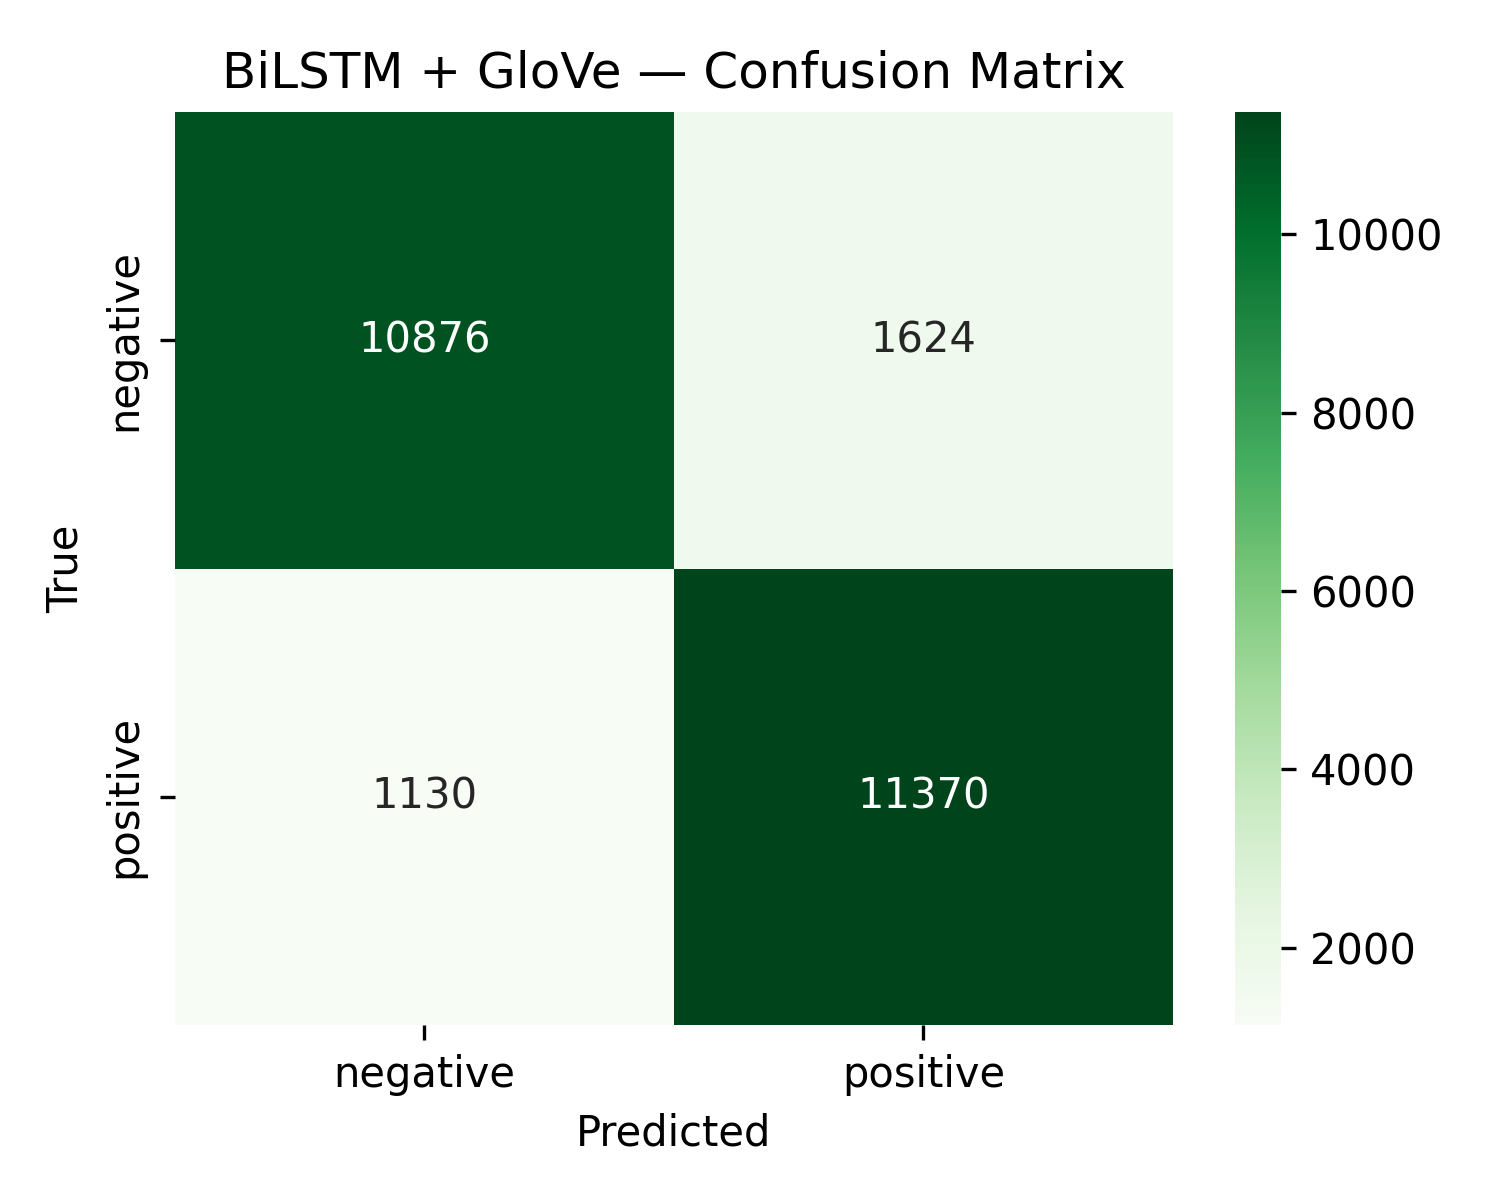
\includegraphics[width=\linewidth]{../q1_classification/outputs/figures/cm_bilstm.png}
	\caption{BiLSTM + GloVe}
\end{subfigure}
\begin{subfigure}{0.32\linewidth}
	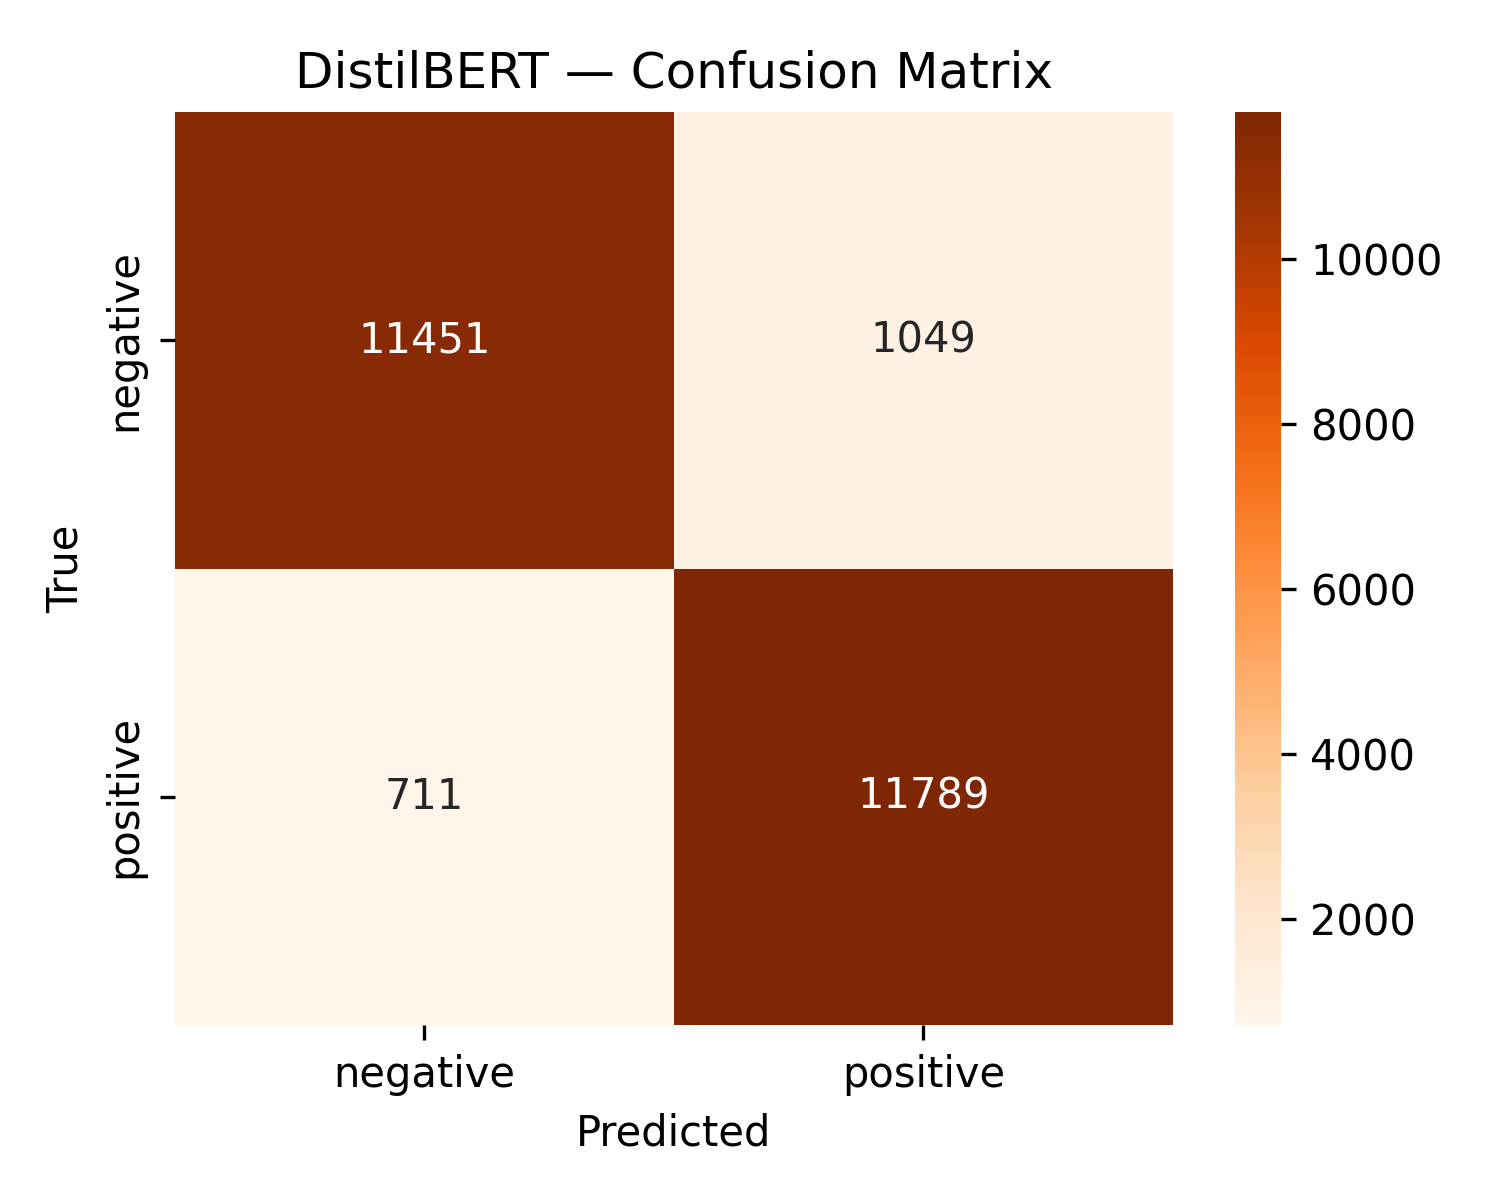
\includegraphics[width=\linewidth]{../q1_classification/outputs/figures/cm_distilbert.png}
	\caption{DistilBERT}
\end{subfigure}
\caption{Confusion matrices for all models.}
\end{figure}

\begin{figure}[H]
\centering
\begin{subfigure}{0.48\linewidth}
	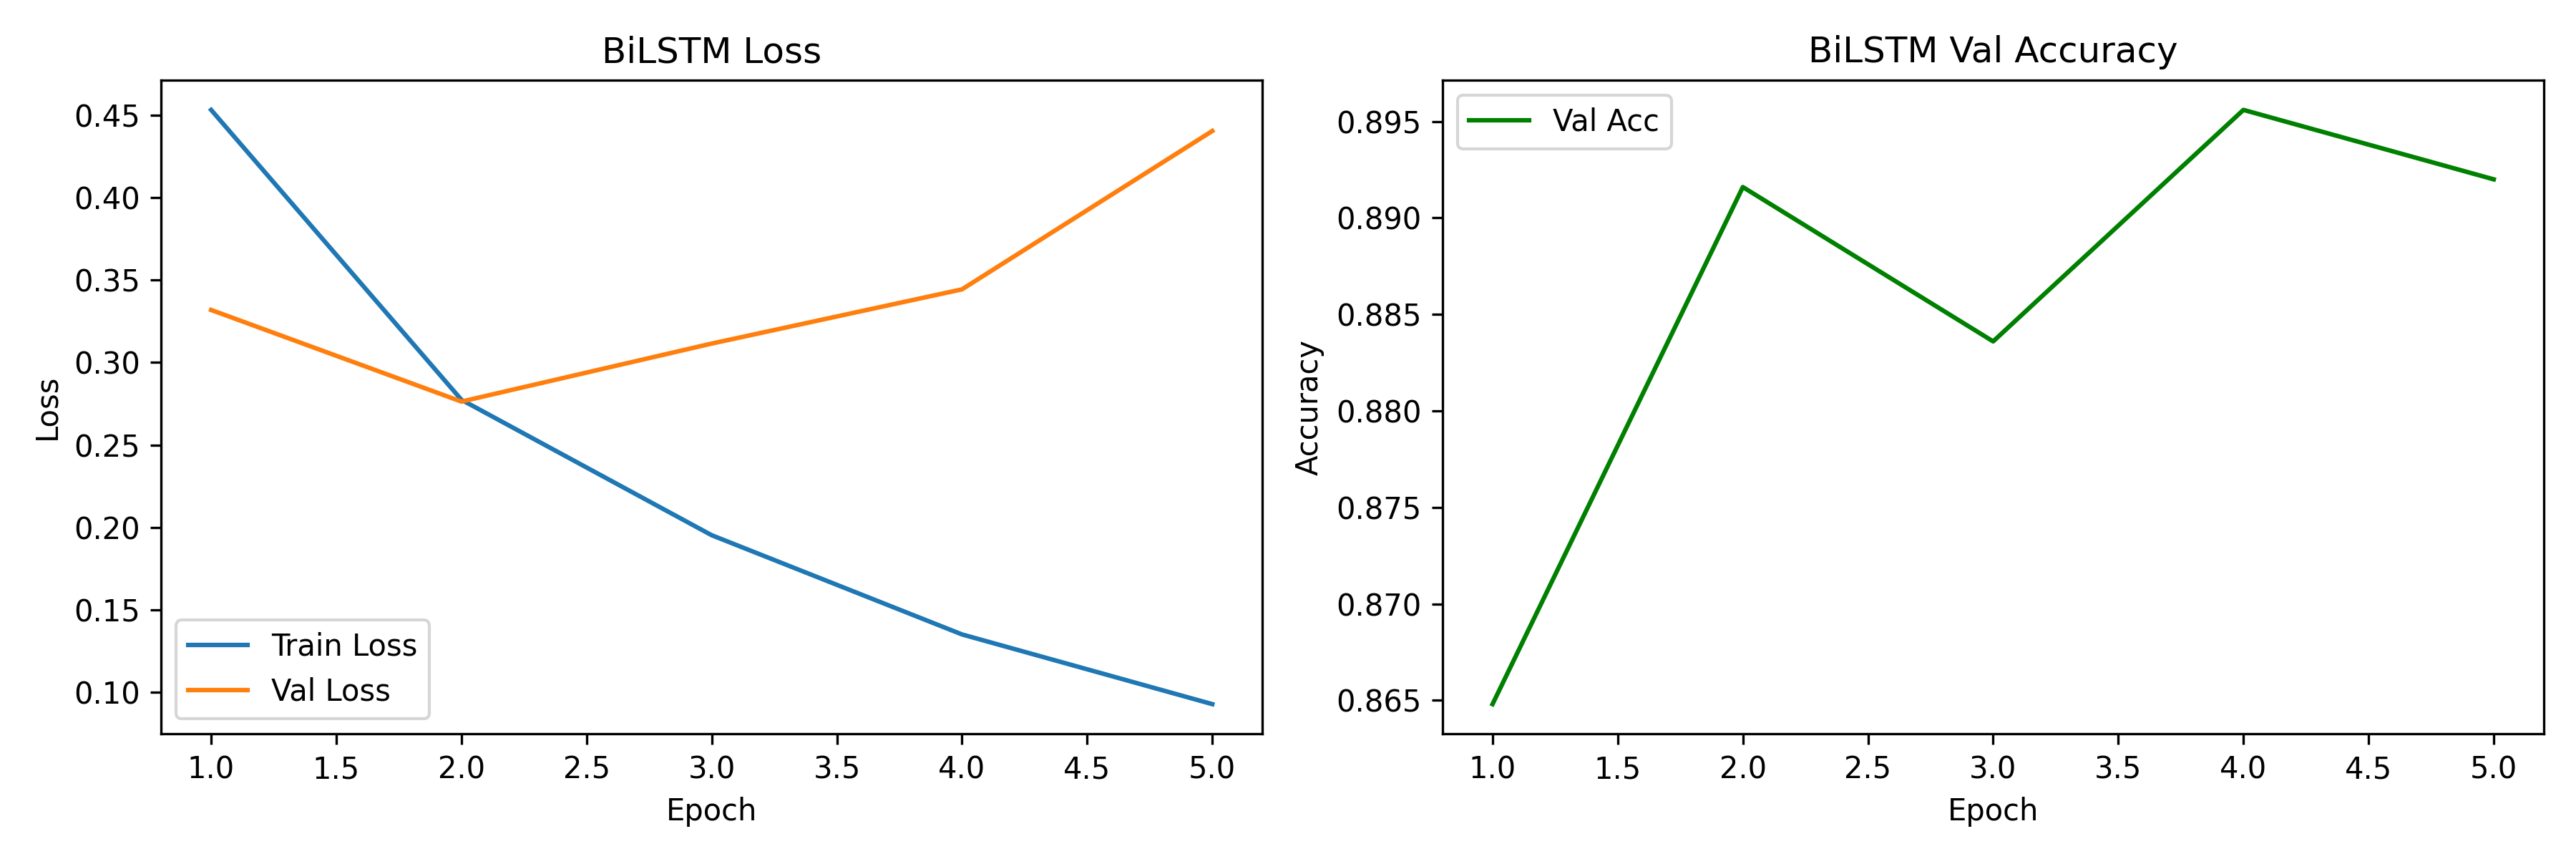
\includegraphics[width=\linewidth]{../q1_classification/outputs/figures/training_bilstm.png}
	\caption{BiLSTM training curves}
\end{subfigure}
\begin{subfigure}{0.48\linewidth}
	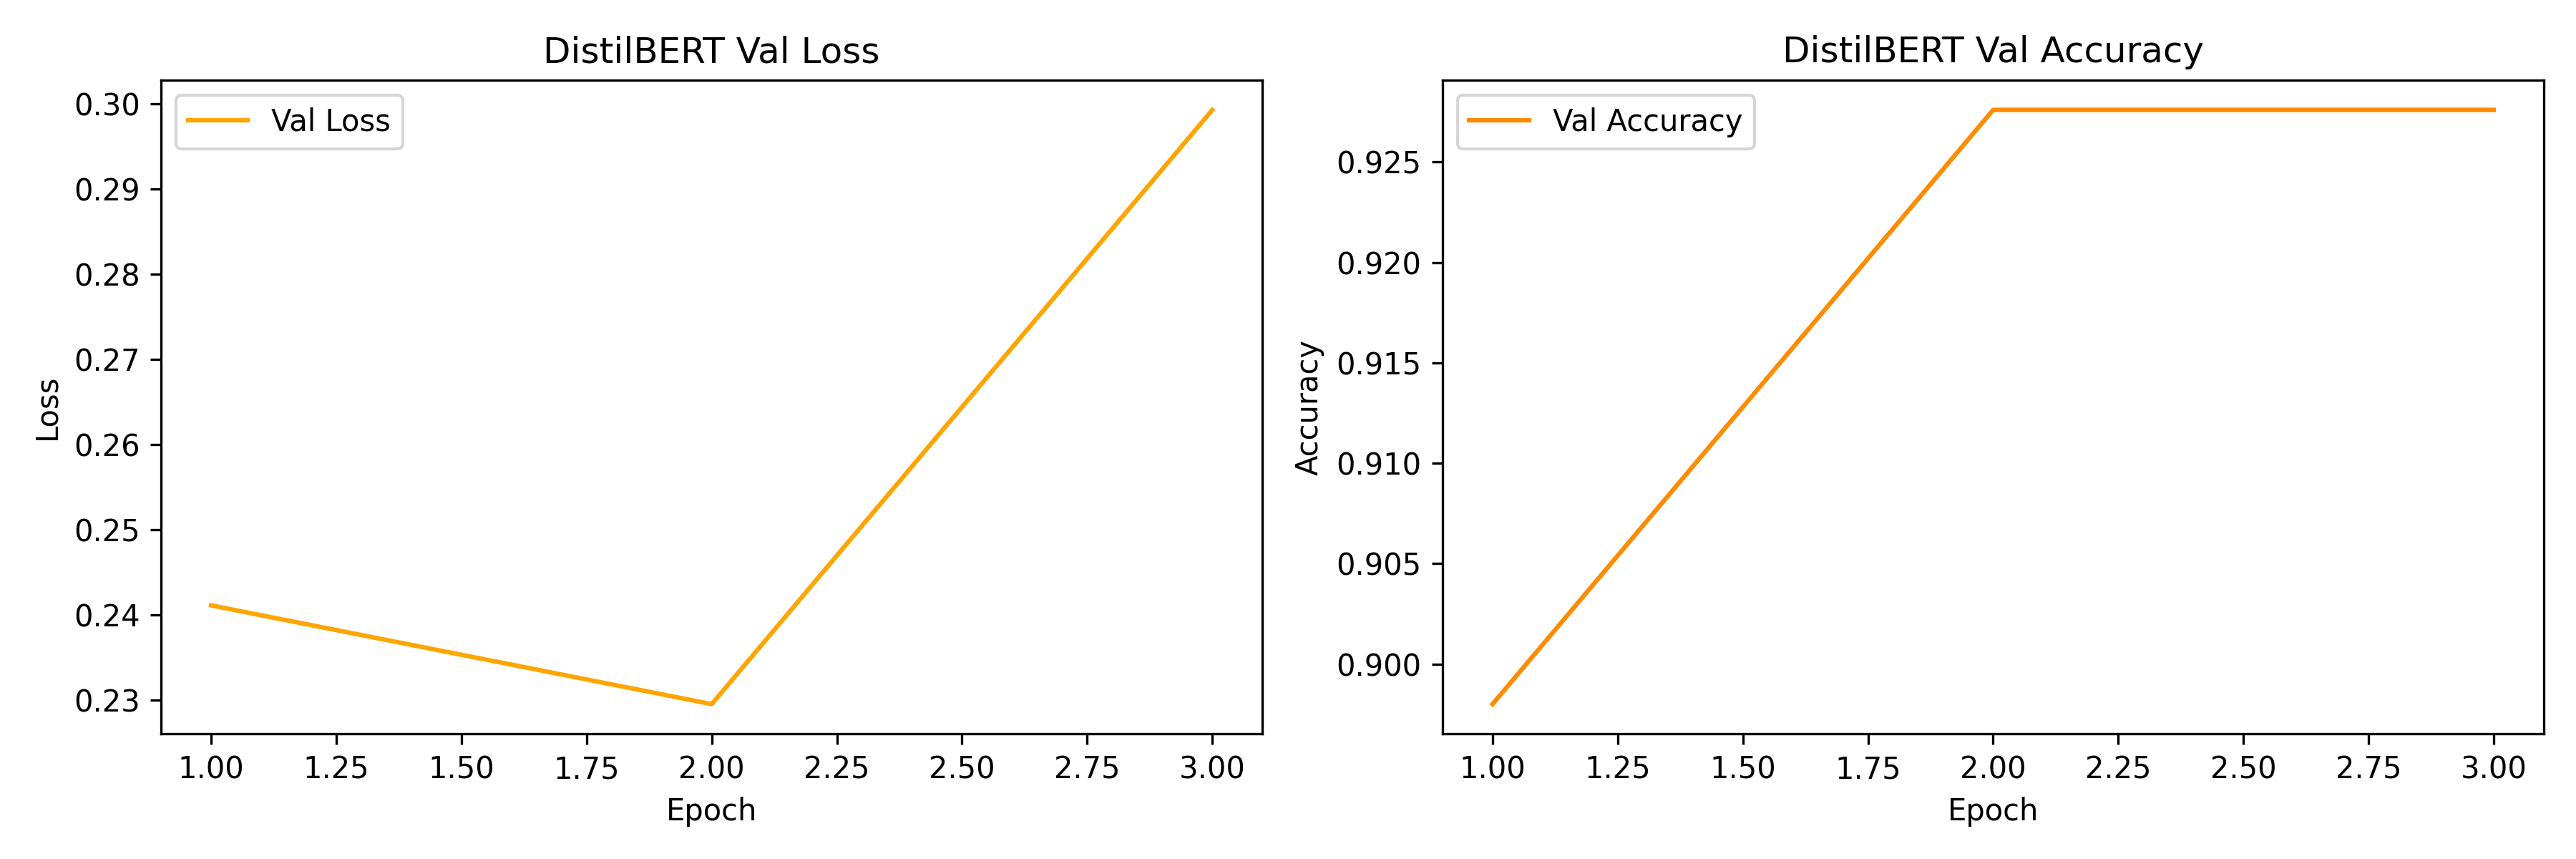
\includegraphics[width=\linewidth]{../q1_classification/outputs/figures/training_distilbert.png}
	\caption{DistilBERT training curves}
\end{subfigure}
\caption{Training dynamics for neural models.}
\end{figure}

\begin{figure}[H]
\centering
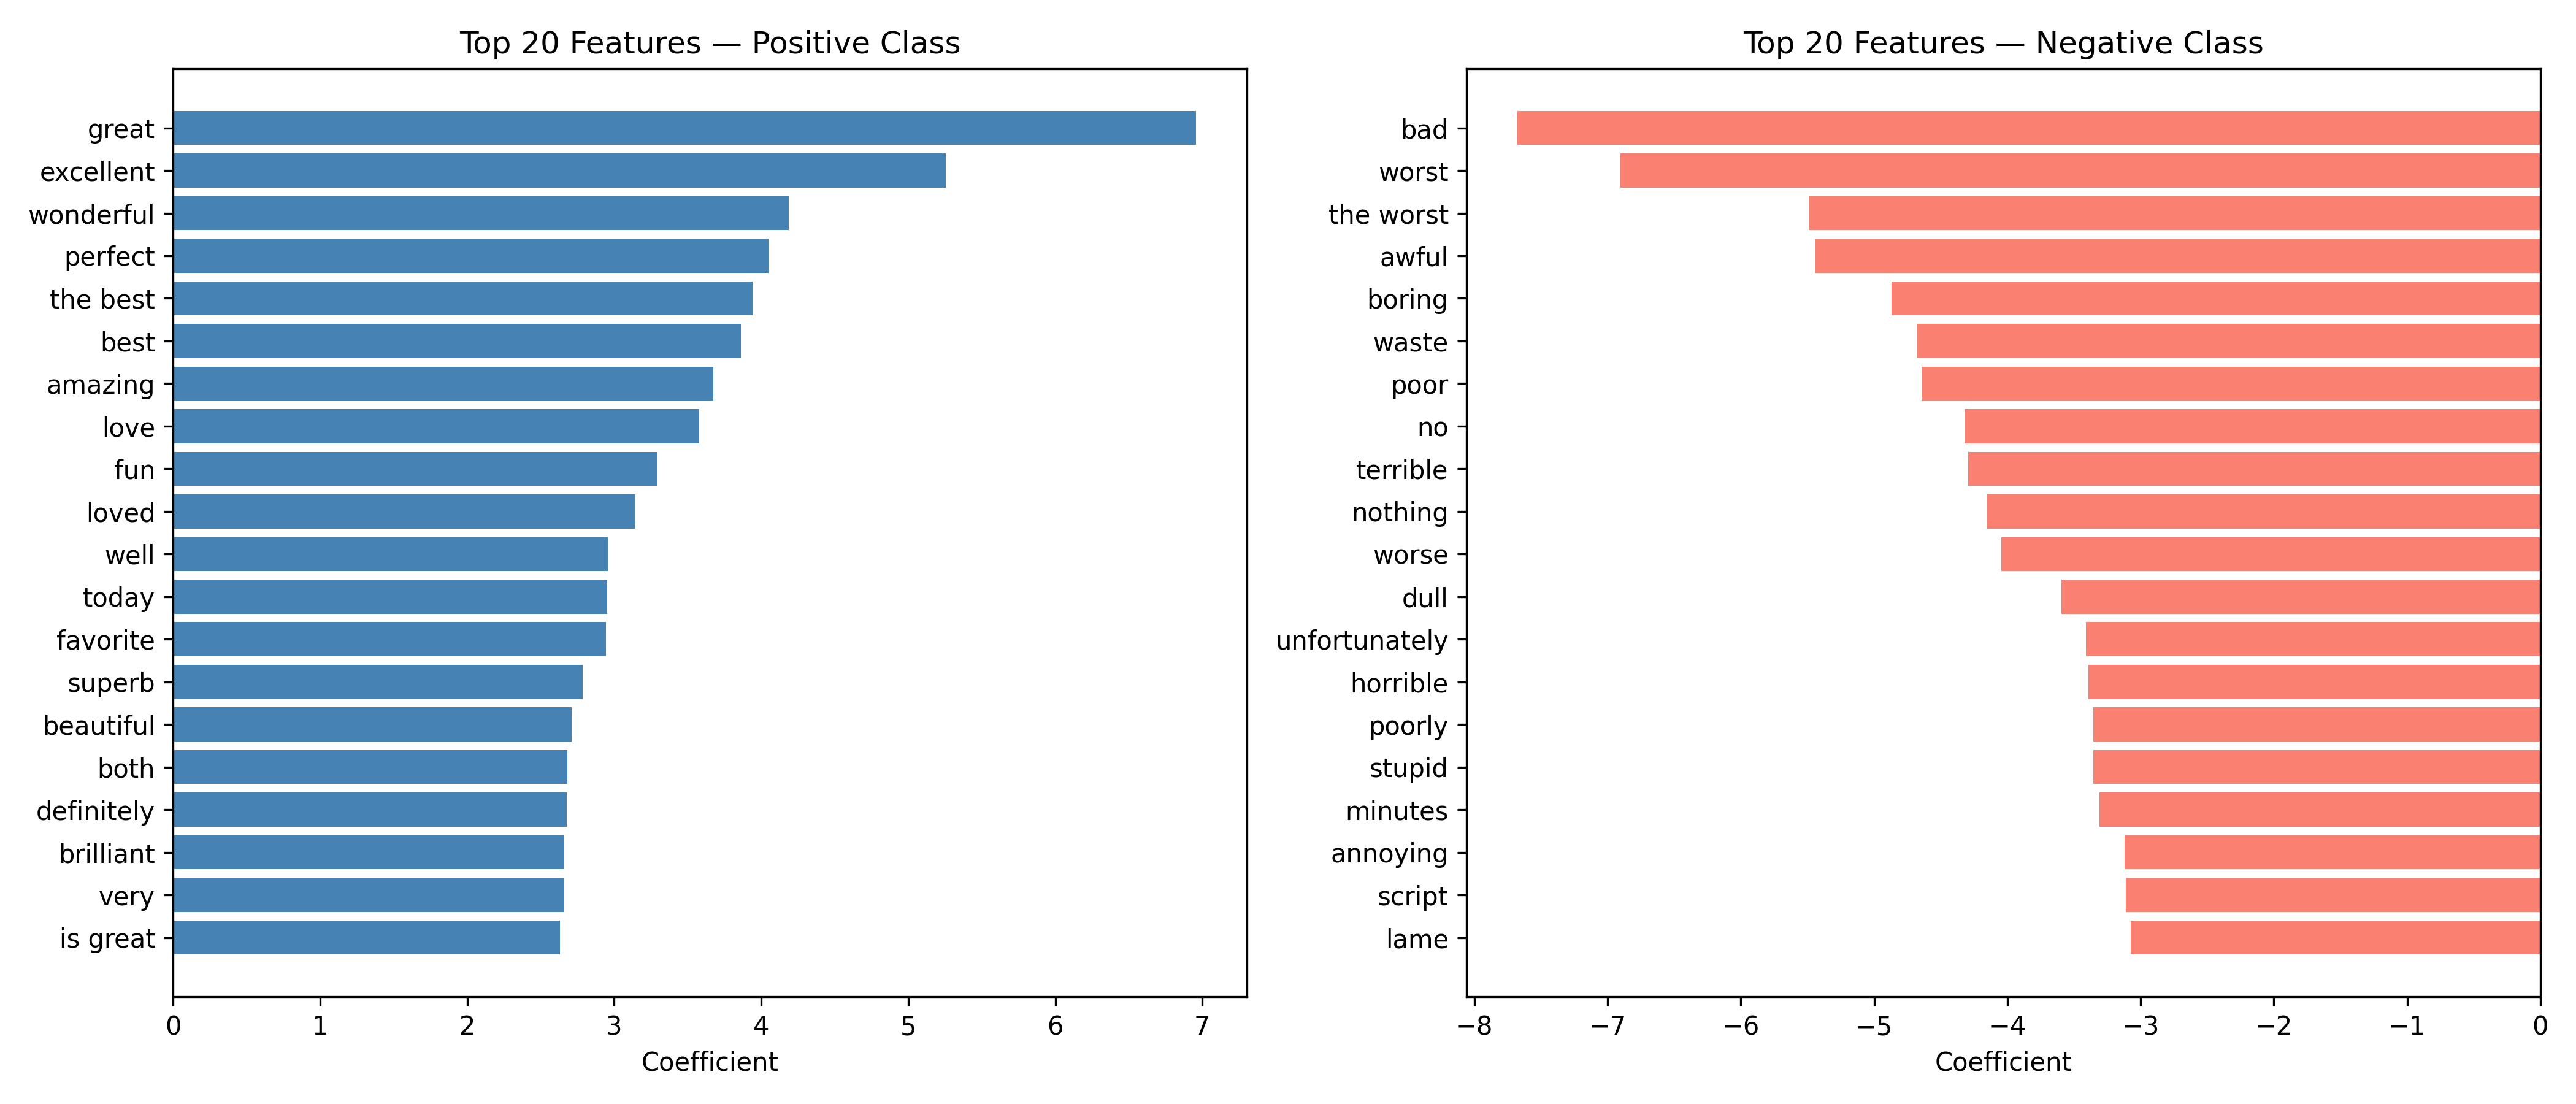
\includegraphics[width=0.9\linewidth]{../q1_classification/outputs/figures/tfidf_features.png}
\caption{Top TF-IDF features for positive and negative classes.}
\end{figure}

\subsection{Error Analysis}
We analyze misclassifications with a focus on common error patterns. The counts are: all three models wrong (774), TF-IDF only wrong (863), BiLSTM only wrong (875), DistilBERT only wrong (512). Five representative errors from the DistilBERT test set include:
\begin{itemize}[leftmargin=*]
		\item \textbf{Negation:} reviews with localized negation often flip sentiment cues (e.g., ``not like this movie").
		\item \textbf{Mixed sentiment:} positive and negative clauses co-occur, making the overall label ambiguous.
		\item \textbf{Domain terms:} film-specific words (e.g., ``plot'', ``acting'') can appear in both positive and negative contexts.
		\item \textbf{Sarcasm:} positive surface words mask negative intent.
		\item \textbf{Subtle tone:} mild criticism or praise without explicit sentiment markers.
\end{itemize}

\subsection{Discussion}
Sparse TF-IDF features are strong for sentiment cues and offer clear interpretability, but they struggle with long-range dependencies and nuanced phrasing. The BiLSTM benefits from sequence modeling but underperforms TF-IDF in this setup, likely due to limited capacity and the difficulty of long reviews. DistilBERT provides the best performance by leveraging contextual embeddings that capture semantics, negation, and long-distance dependencies more effectively, at the cost of higher training time and lower transparency.


% ── Q2 ────────────────────────────────────────────────────────────────────────
\newpage
\section{Question 2: Named Entity Recognition}
% Q2 NER section

\subsection{Problem Formulation}
Named Entity Recognition (NER) is a sequence labeling task. Given a token sequence $x = (x_1, \dots, x_n)$, the model predicts a BIO tag sequence $y = (y_1, \dots, y_n)$, where each $y_i \in \{\texttt{O}, \texttt{B-}t, \texttt{I-}t\}$ and $t \in \{\texttt{PER}, \texttt{ORG}, \texttt{LOC}, \texttt{MISC}\}$. We evaluate entity-level precision, recall, and F1 using the \texttt{seqeval} metric.

\subsection{Dataset Description}
We use the CoNLL-2003 dataset with official train/validation/test splits. The label inventory contains 9 BIO tags: \texttt{O}, \texttt{B/I-PER}, \texttt{B/I-ORG}, \texttt{B/I-LOC}, \texttt{B/I-MISC}.

\begin{table}[H]
\centering
\caption{CoNLL-2003 dataset statistics.}
\begin{tabular}{lrrrr}
\toprule
\textbf{Split} & \textbf{Sentences} & \textbf{Tokens} & \textbf{Avg Len} & \textbf{Entity \%} \\
\midrule
Train & 14,041 & 203,621 & 14.50 & 16.72 \\
Validation & 3,250 & 51,362 & 15.80 & 16.75 \\
Test & 3,453 & 46,435 & 13.45 & 17.47 \\
\bottomrule
\end{tabular}
\end{table}

\begin{table}[H]
\centering
\caption{Entity token counts per split.}
\begin{tabular}{lrrrr}
\toprule
\textbf{Split} & \textbf{PER} & \textbf{ORG} & \textbf{LOC} & \textbf{MISC} \\
\midrule
Train & 11,128 & 10,025 & 8,297 & 4,593 \\
Validation & 3,149 & 2,092 & 2,094 & 1,268 \\
Test & 2,773 & 2,496 & 1,925 & 918 \\
\bottomrule
\end{tabular}
\end{table}

\subsection{Methodology}
\textbf{BiLSTM-CRF.} We build a word-level vocabulary (20k) and a character vocabulary, initialize word embeddings with GloVe 100d, and use a character BiLSTM to produce subword-aware representations. The final architecture is word+char embeddings $\rightarrow$ BiLSTM $\rightarrow$ linear layer $\rightarrow$ CRF. The CRF models label dependencies and enforces BIO-consistent transitions.

\textbf{BERT token classification.} We use \texttt{bert-base-cased} with a token classification head. Because BERT uses WordPiece tokenization, we align labels by assigning the original label to the first subword and \texttt{-100} to subsequent subwords and special tokens (ignored in the loss). We train for 3 epochs with batch size 16 and learning rate $5\times10^{-5}$.

\subsection{Experimental Setup}
We fix the random seed to 42 and evaluate once on the test split. Early stopping is applied to BiLSTM-CRF based on validation F1 (patience 5). The BERT training time is 138.23 seconds; BiLSTM-CRF timing was logged as 0.0 seconds in the output (likely a timing artifact).

\subsection{Results}
\begin{table}[H]
\centering
\caption{Per-entity and overall results on the test set.}
\begin{tabular}{llccc}
\toprule
\textbf{Entity} & \textbf{Model} & \textbf{Precision} & \textbf{Recall} & \textbf{F1} \\
\midrule
PER & BiLSTM-CRF & 0.9363 & 0.9091 & 0.9225 \\
PER & BERT & 0.9645 & 0.9591 & 0.9618 \\
ORG & BiLSTM-CRF & 0.8712 & 0.8104 & 0.8397 \\
ORG & BERT & 0.8733 & 0.9043 & 0.8885 \\
LOC & BiLSTM-CRF & 0.8972 & 0.9107 & 0.9039 \\
LOC & BERT & 0.9324 & 0.9268 & 0.9296 \\
MISC & BiLSTM-CRF & 0.7356 & 0.7849 & 0.7595 \\
MISC & BERT & 0.7691 & 0.8162 & 0.7920 \\
\midrule
Overall & BiLSTM-CRF & 0.8793 & 0.8651 & 0.8721 \\
Overall & BERT & 0.9024 & 0.9157 & 0.9090 \\
\bottomrule
\end{tabular}
\end{table}

\begin{figure}[H]
\centering
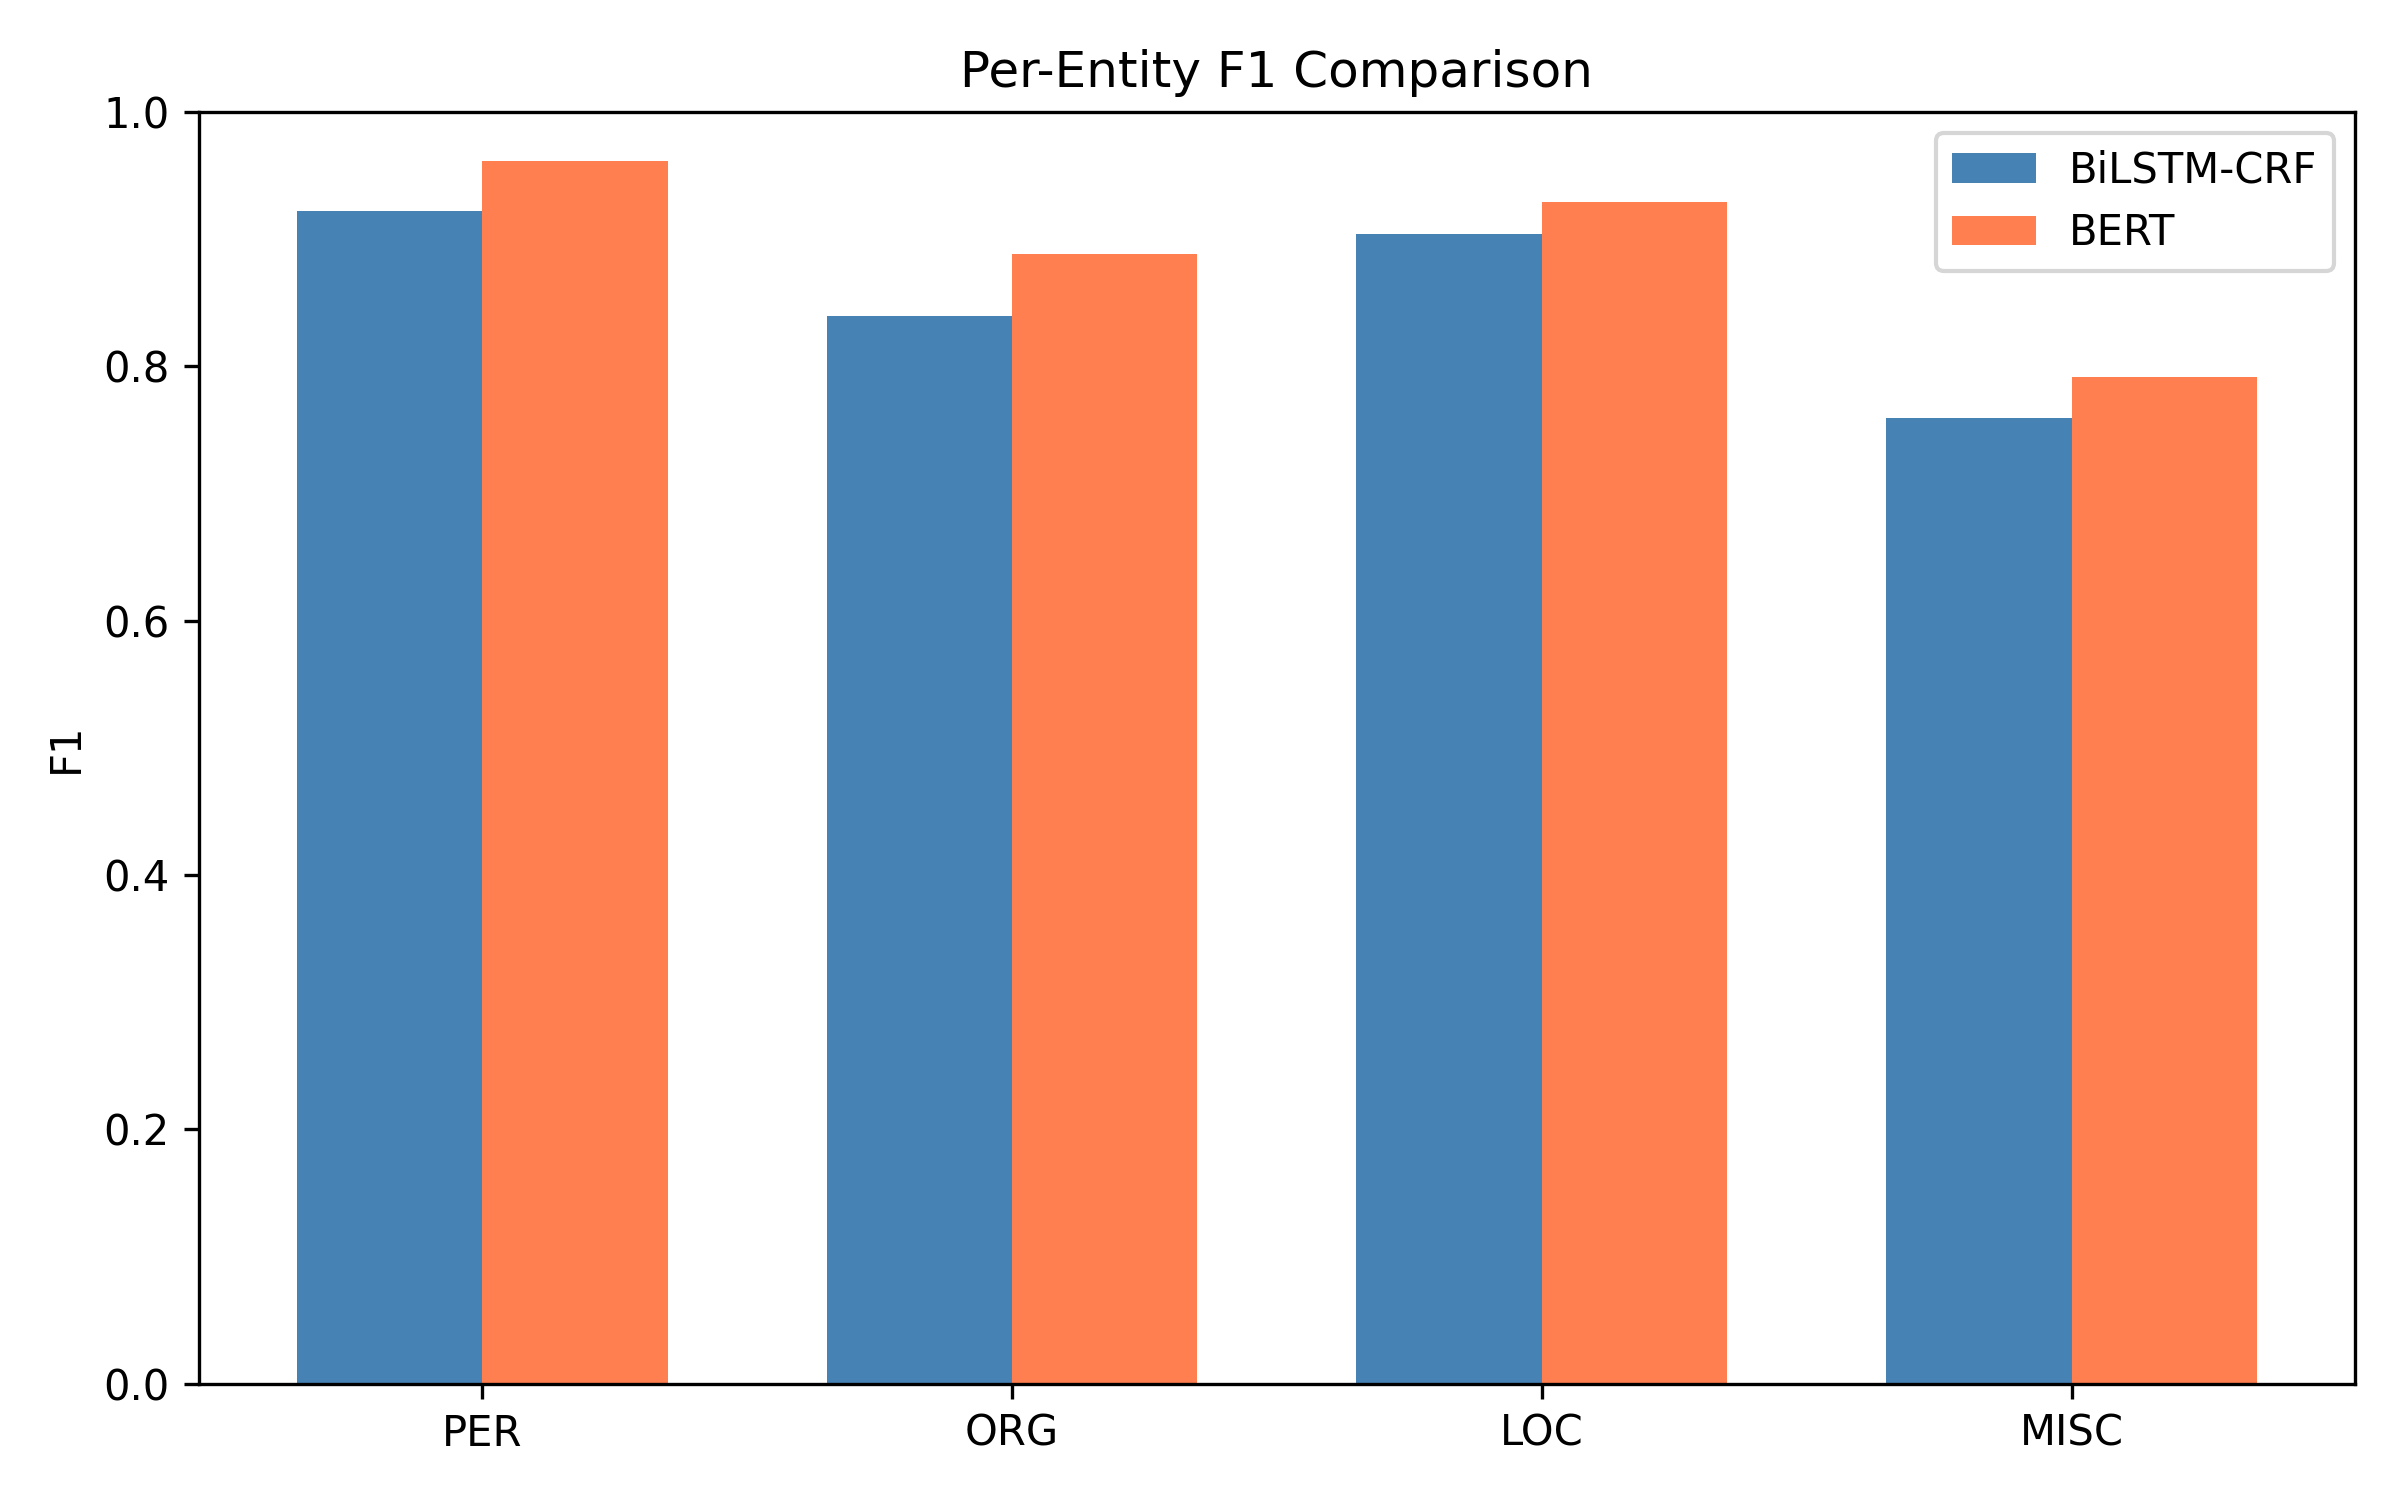
\includegraphics[width=0.75\linewidth]{../q2_ner/outputs/figures/per_entity_f1.png}
\caption{Per-entity F1 comparison between BiLSTM-CRF and BERT.}
\end{figure}

\begin{figure}[H]
\centering
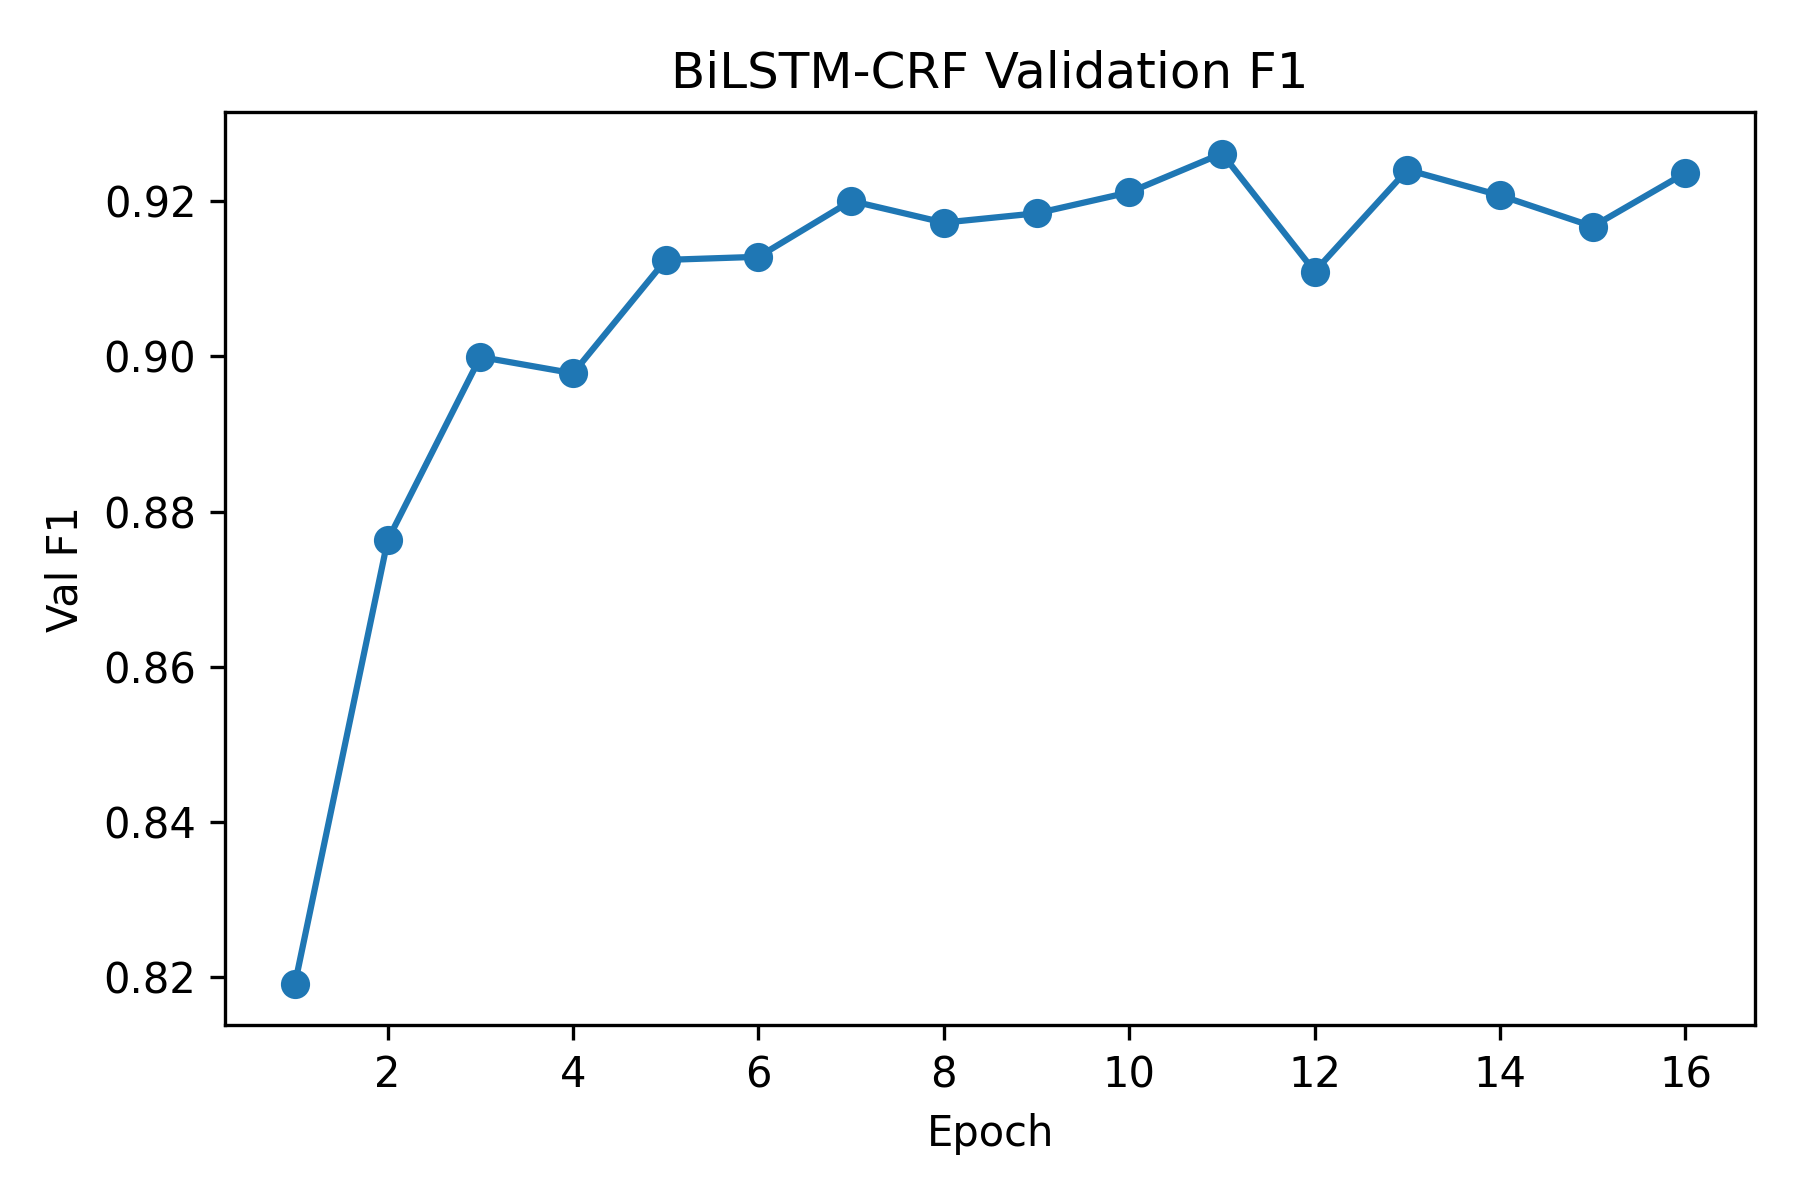
\includegraphics[width=0.65\linewidth]{../q2_ner/outputs/figures/training_bilstm_crf.png}
\caption{BiLSTM-CRF validation F1 across epochs.}
\end{figure}

\begin{figure}[H]
\centering
\begin{subfigure}{0.48\linewidth}
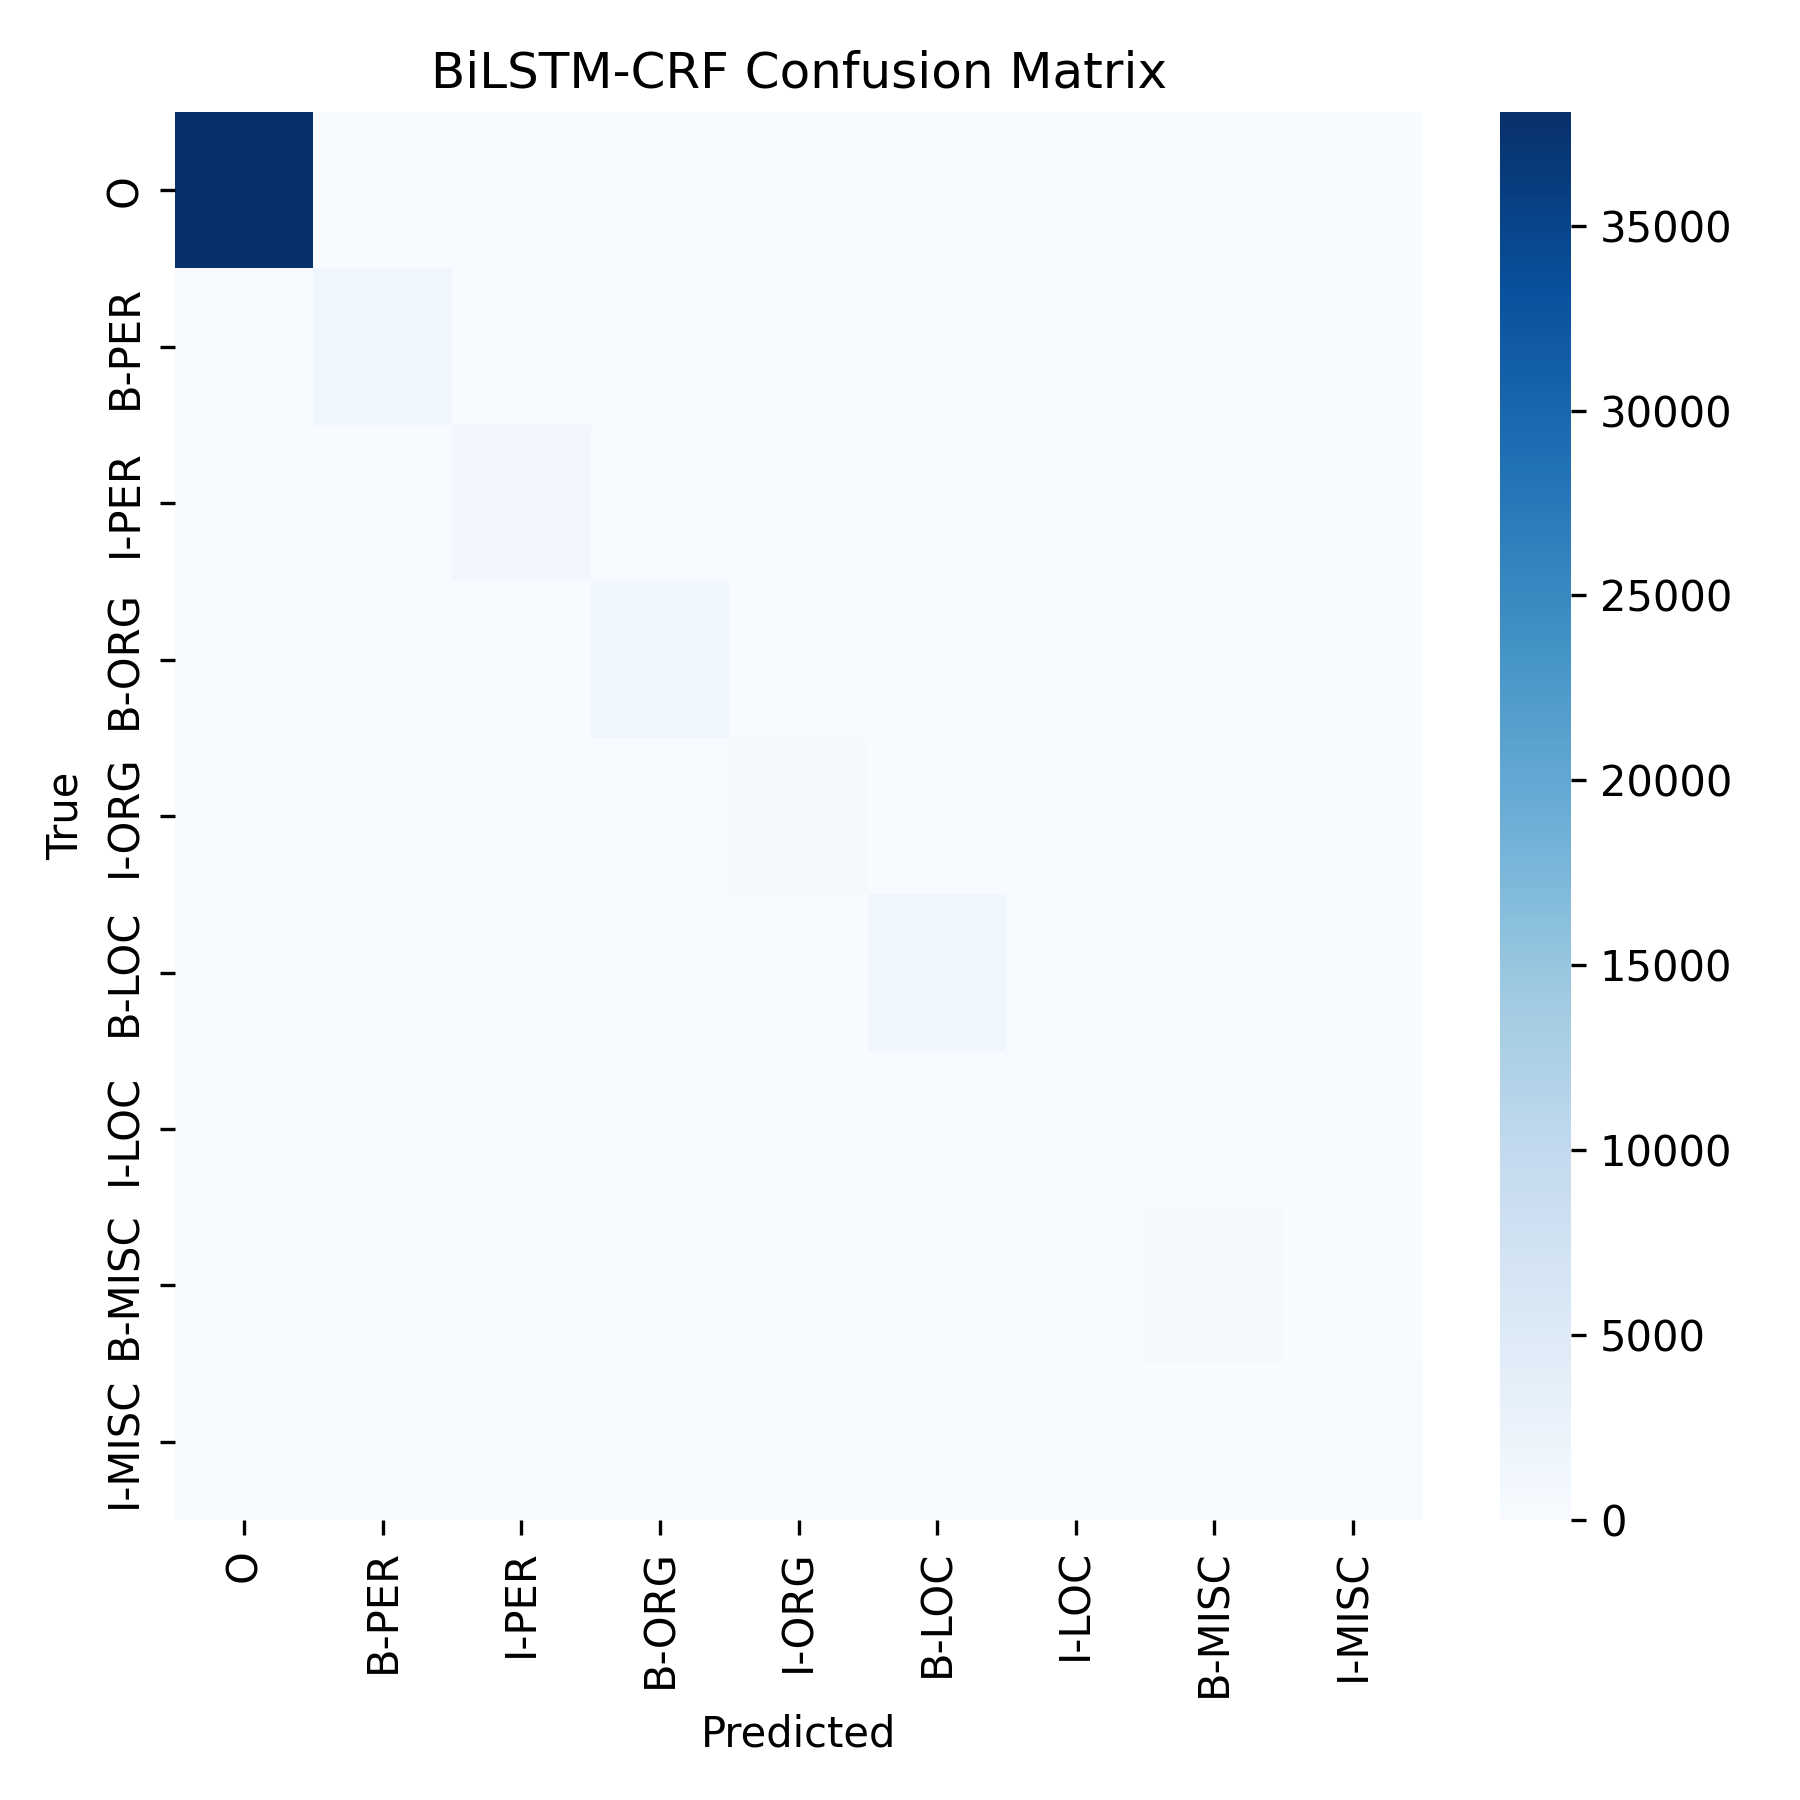
\includegraphics[width=\linewidth]{../q2_ner/outputs/figures/cm_bilstm_crf.png}
\caption{BiLSTM-CRF}
\end{subfigure}
\begin{subfigure}{0.48\linewidth}
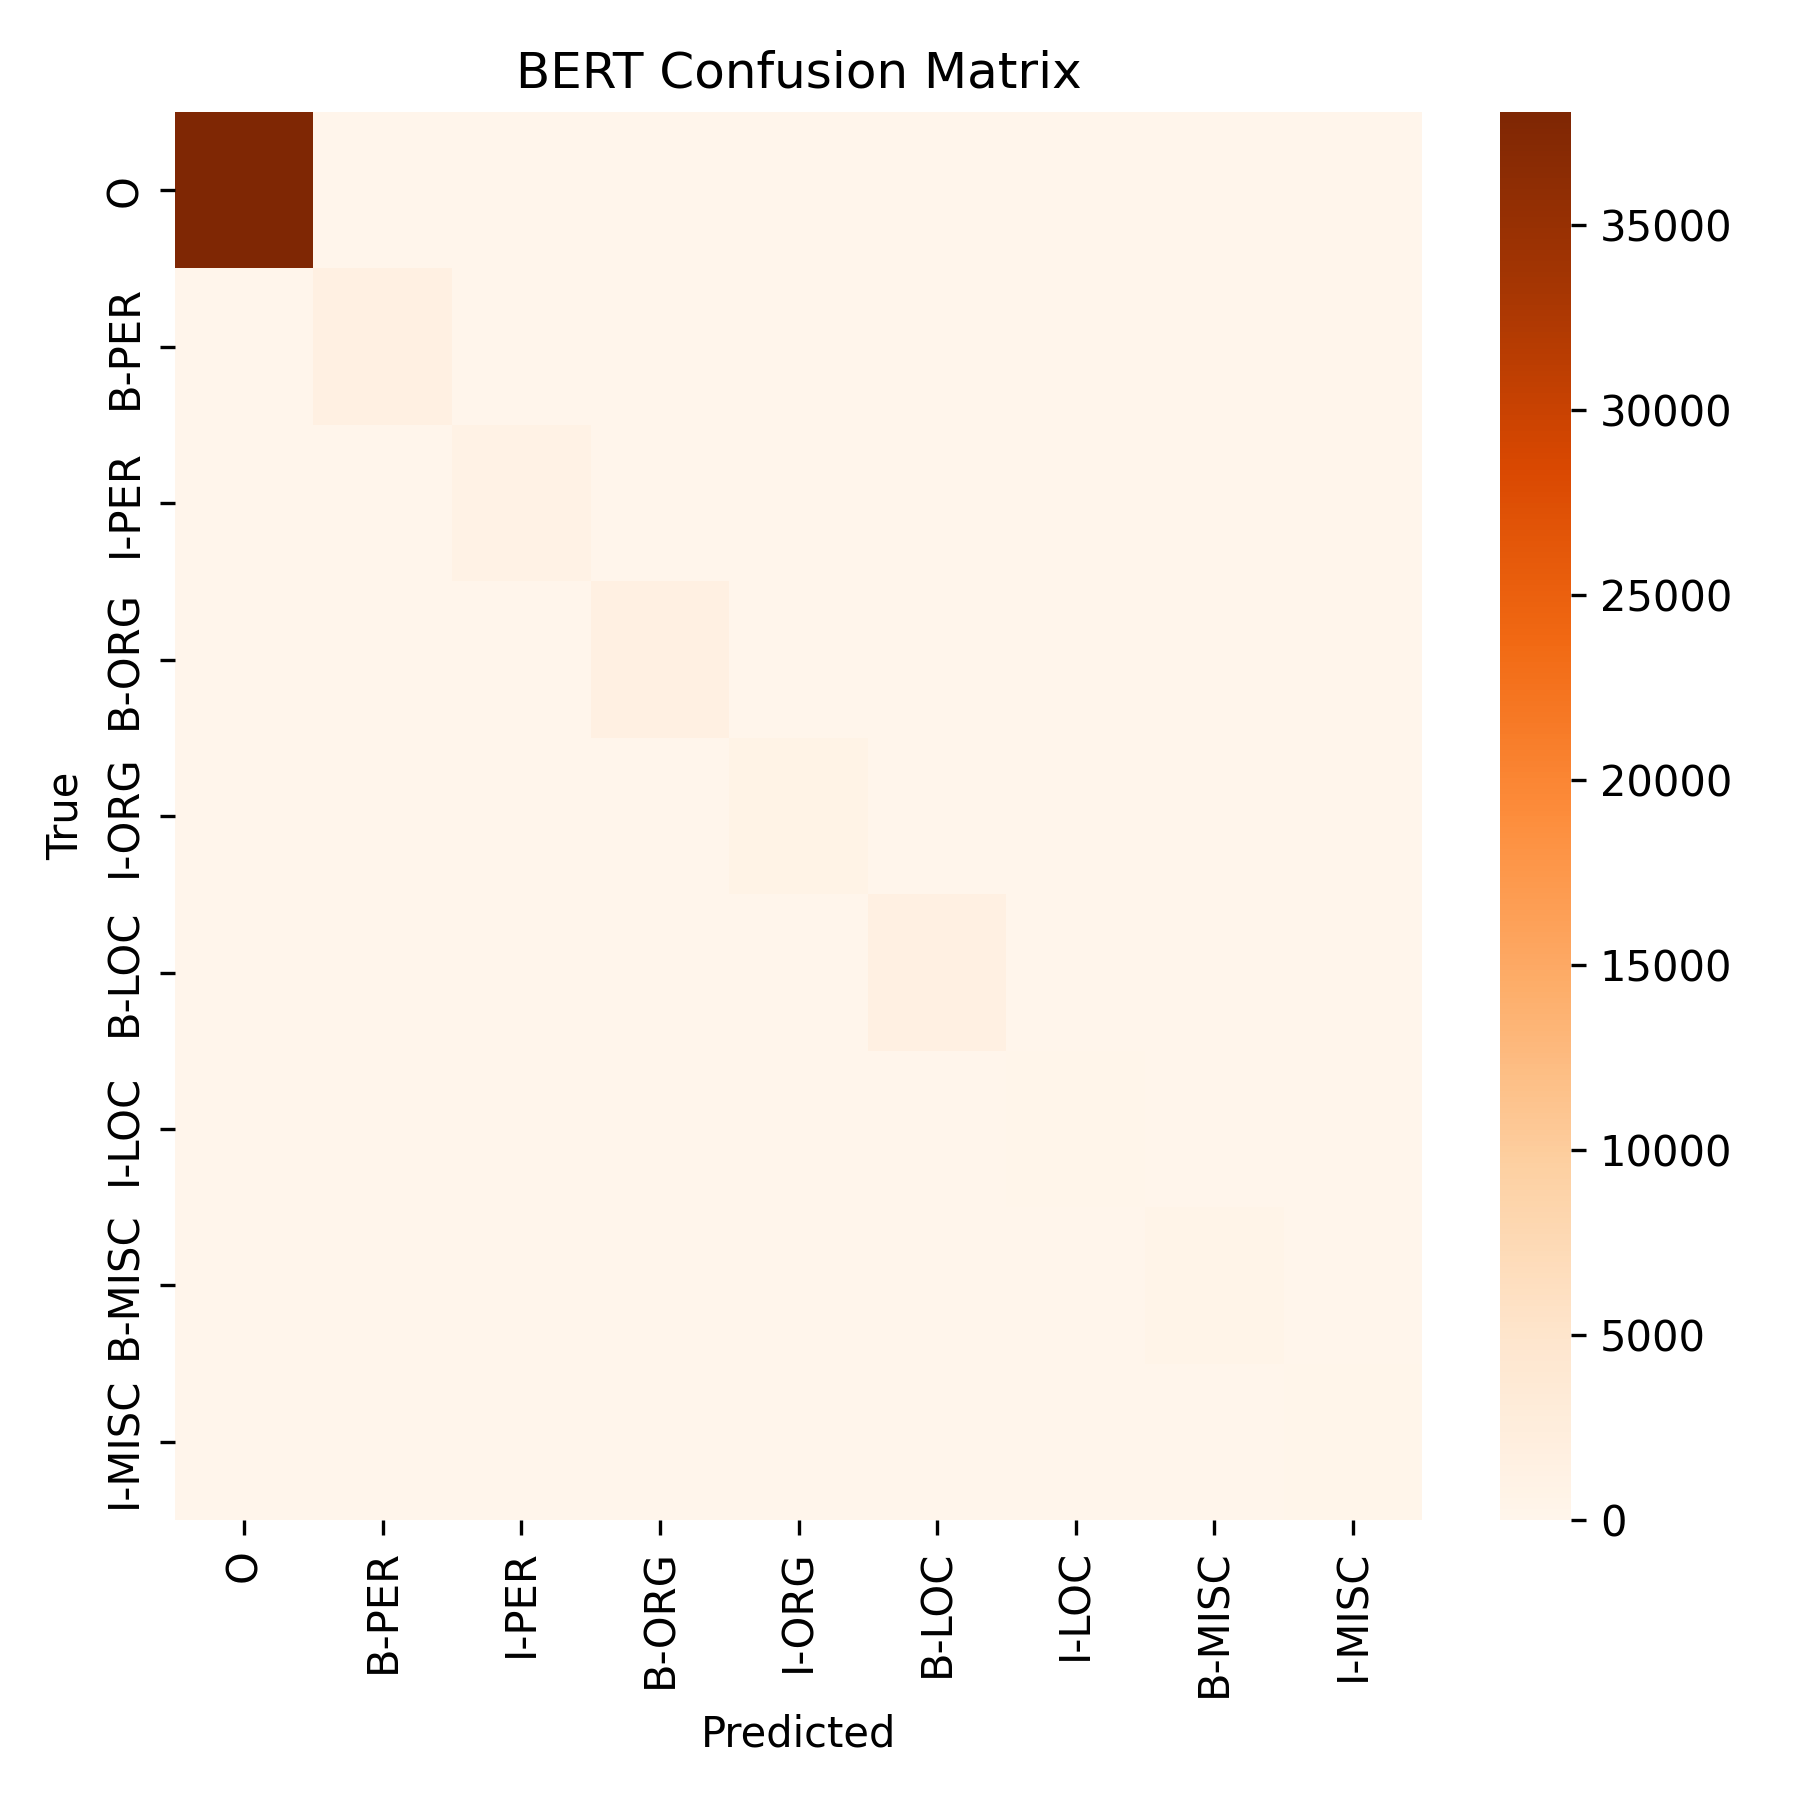
\includegraphics[width=\linewidth]{../q2_ner/outputs/figures/cm_bert.png}
\caption{BERT}
\end{subfigure}
\caption{Confusion matrices over BIO labels.}
\end{figure}

\begin{figure}[H]
\centering
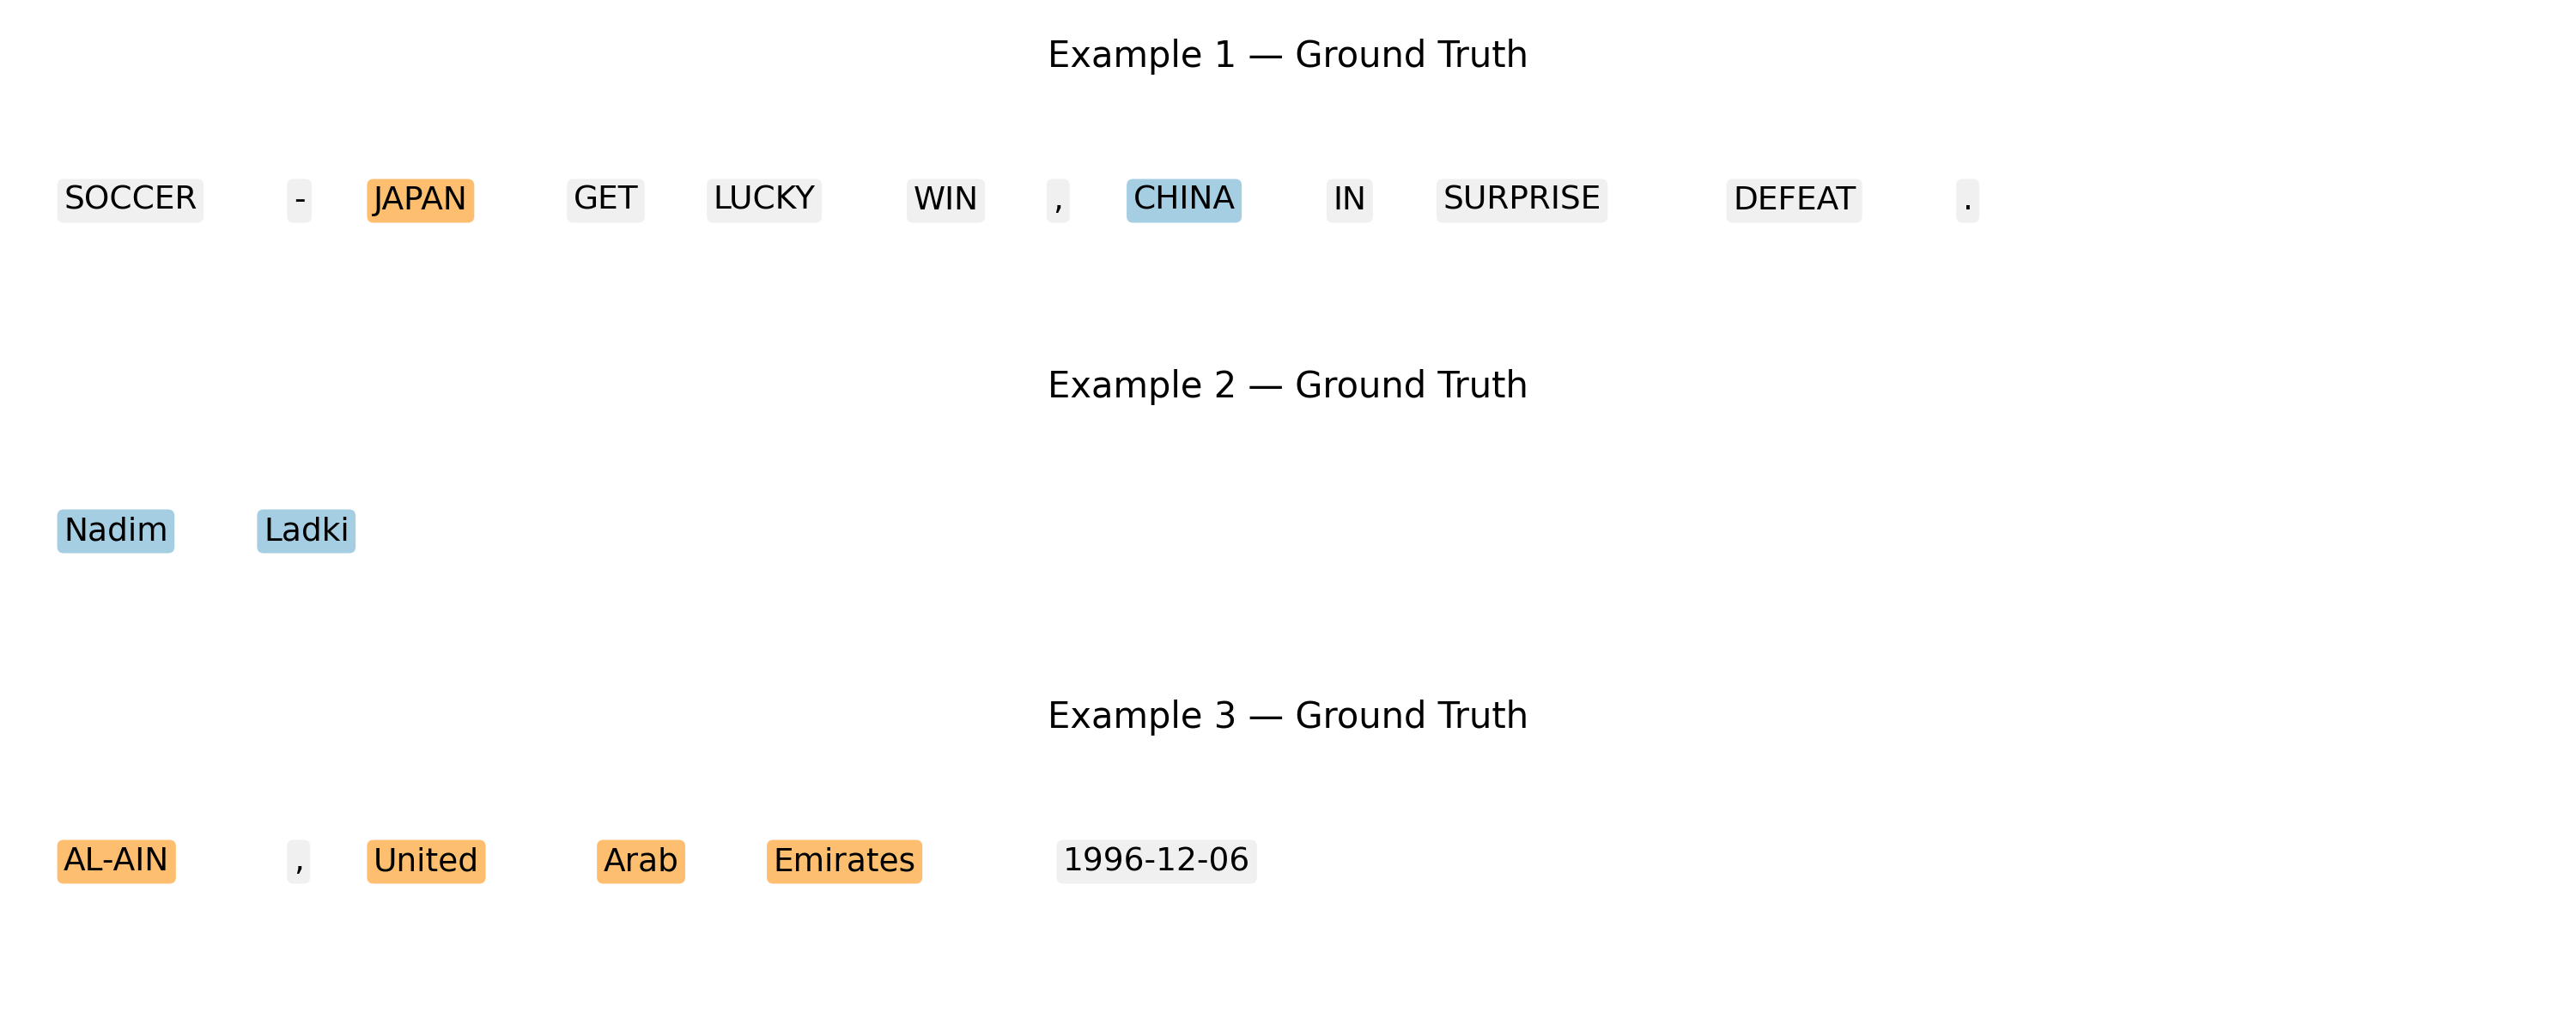
\includegraphics[width=0.90\linewidth]{../q2_ner/outputs/figures/entity_examples.png}
\caption{Example sentences with gold entity labels.}
\end{figure}

\subsection{Error Analysis}
We categorize errors using span-level comparisons on BERT predictions. The counts are: type confusion (317), false positives (139), boundary errors (81), and false negatives (74). Five representative errors are:

\begin{itemize}[leftmargin=*]
\item \textbf{Type confusion (LOC $\rightarrow$ ORG/PER).} Sentence: \texttt{SOCCER - JAPAN GET LUCKY WIN , CHINA IN SURPRISE DEFEAT .} \\ True: \texttt{O O B-LOC O O O O B-PER O O O O} \\ Pred: \texttt{O O B-ORG O O O O B-ORG O O O O}. \\ Hypothesis: country names in sports headlines are often interpreted as organizations.
\item \textbf{False negative (missed PER/LOC).} Sentence: \texttt{RUGBY UNION - CUTTITTA BACK FOR ITALY AFTER A YEAR .} \\ True: \texttt{B-ORG I-ORG O B-PER O O B-LOC O O O O} \\ Pred: \texttt{B-ORG I-ORG O B-ORG O O O O O O O}. \\ Hypothesis: person names in uppercase are confused with organizations, and nearby locations are dropped.
\item \textbf{Boundary error (missing initial token).} Sentence: \texttt{Cuttitta announced his retirement after the 1995 World Cup , ...} \\ True: \texttt{B-PER ... B-MISC I-MISC I-MISC ...} \\ Pred: \texttt{B-PER ... O B-MISC I-MISC ...}. \\ Hypothesis: multi-token event names are truncated.
\item \textbf{Boundary error (invalid BIO start).} Sentence: \texttt{FREESTYLE SKIING-WORLD CUP MOGUL RESULTS .} \\ True: \texttt{O B-MISC I-MISC O O O} \\ Pred: \texttt{O O I-MISC O O O}. \\ Hypothesis: model sometimes emits \texttt{I-} without a preceding \texttt{B-} for hyphenated entities.
\item \textbf{False positive (spurious MISC).} Sentence: \texttt{CRICKET - LARA SUFFERS MORE AUSTRALIAN TOUR MISERY .} \\ True: \texttt{O O B-PER O O O O O O} \\ Pred: \texttt{O O B-MISC O O B-MISC O I-MISC O}. \\ Hypothesis: sports-related phrases are over-labeled as \texttt{MISC}.
\end{itemize}

\subsection{Discussion}
BERT outperforms BiLSTM-CRF overall (0.909 vs 0.872 F1) and across all entity types, with the largest gains on PER and ORG. Both models struggle most with MISC, indicating weaker boundaries for heterogeneous categories. The dominant error type is label confusion, suggesting that headline-style contexts and uppercase tokens blur distinctions between LOC, ORG, and PER. Incorporating gazetteers or additional contextual features could reduce these confusions.


% ── Q3 ────────────────────────────────────────────────────────────────────────
\newpage
\section{Question 3: Text Summarization}
% Q3 summarization section

\subsection{Problem Formulation}
We study text summarization on CNN/DailyMail and compare extractive methods (selecting sentences) against abstractive methods (generating new text). Given an article $x$, the system outputs a summary $\hat{y}$ that should be fluent, faithful to the source, and cover the main points. We evaluate with ROUGE, BLEU, METEOR, and BERTScore.

\subsection{Dataset Description}
CNN/DailyMail \citep{Hermann2015cnndm} (version 3.0.0) provides news articles with reference highlights. We use a subset for tractable computation.

\begin{table}[H]
\centering
\caption{CNN/DailyMail dataset statistics.}
\begin{tabular}{lrr}
\toprule
\textbf{Split} & \textbf{Original Size} & \textbf{Subset Size} \\
\midrule
Train & 287,113 & 10,000 \\
Validation & 13,368 & 1,000 \\
Test & 11,490 & 1,000 \\
\bottomrule
\end{tabular}
\end{table}

\begin{table}[H]
\centering
\caption{Average document statistics (computed on test subset).}
\begin{tabular}{lrrrr}
\toprule
\textbf{Avg Article Len (words)} & \textbf{Avg Summary Len (words)} & \textbf{Avg Sentences} & \textbf{Compression Ratio} \\
\midrule
676.08 & 55.21 & 32.91 & 12.25 \\
\bottomrule
\end{tabular}
\end{table}

\subsection{Methodology}
\textbf{Extractive (TextRank, LexRank).} Both algorithms build a sentence similarity graph and rank sentences by centrality. The summary is formed by selecting the top-$k$ sentences (here $k=3$). TextRank \citep{MihalceaTarau2004textrank} uses a PageRank-style score on sentence similarity, while LexRank \citep{ErkanRadev2004lexrank} adds an explicit cosine similarity graph with thresholding.

\textbf{Abstractive (BART, T5).} We use encoder-decoder transformers. BART-large-cnn \citep{Lewis2020bart} is fine-tuned for summarization and generates fluent, condensed summaries. T5-small \citep{Raffel2020t5} is prompted with a ``summarize:'' prefix and generates shorter, more compressed outputs. ROUGE \citep{Lin2004rouge}, METEOR \citep{BanerjeeLavie2005meteor}, BLEU \citep{Papineni2002bleu}, and BERTScore \citep{Zhang2020bertscore} are reported as complementary metrics: ROUGE/BLEU measure n-gram overlap, METEOR adds stem and synonym matching, and BERTScore uses contextual embeddings.

\subsection{Experimental Setup}
All runs use a fixed seed (42). Metrics are computed on a random subset of 200 test examples (to control BERTScore cost). We report average inference time per article for each method.

\subsection{Results}
\begin{table}[H]
\centering
\caption{Summarization metrics (evaluation size = 200).}
\begin{tabular}{lrrrrrrrr}
\toprule
\textbf{Method} & \textbf{R-1} & \textbf{R-2} & \textbf{R-L} & \textbf{BLEU} & \textbf{METEOR} & \textbf{BERT F1} & \textbf{Len} & \textbf{ms} \\
\midrule
TextRank & 0.3361 & 0.1329 & 0.2155 & 0.0728 & 0.3020 & 0.8623 & 96.00 & 62.51 \\
LexRank & 0.3501 & 0.1340 & 0.2195 & 0.0827 & 0.2806 & 0.8650 & 74.17 & 60.68 \\
BART & 0.4375 & 0.2166 & 0.3148 & 0.1467 & 0.3308 & 0.8826 & 61.28 & 898.39 \\
T5 & 0.3795 & 0.1747 & 0.2683 & 0.1030 & 0.2531 & 0.8680 & 46.25 & 188.26 \\
\bottomrule
\end{tabular}
\end{table}

\begin{figure}[H]
\centering
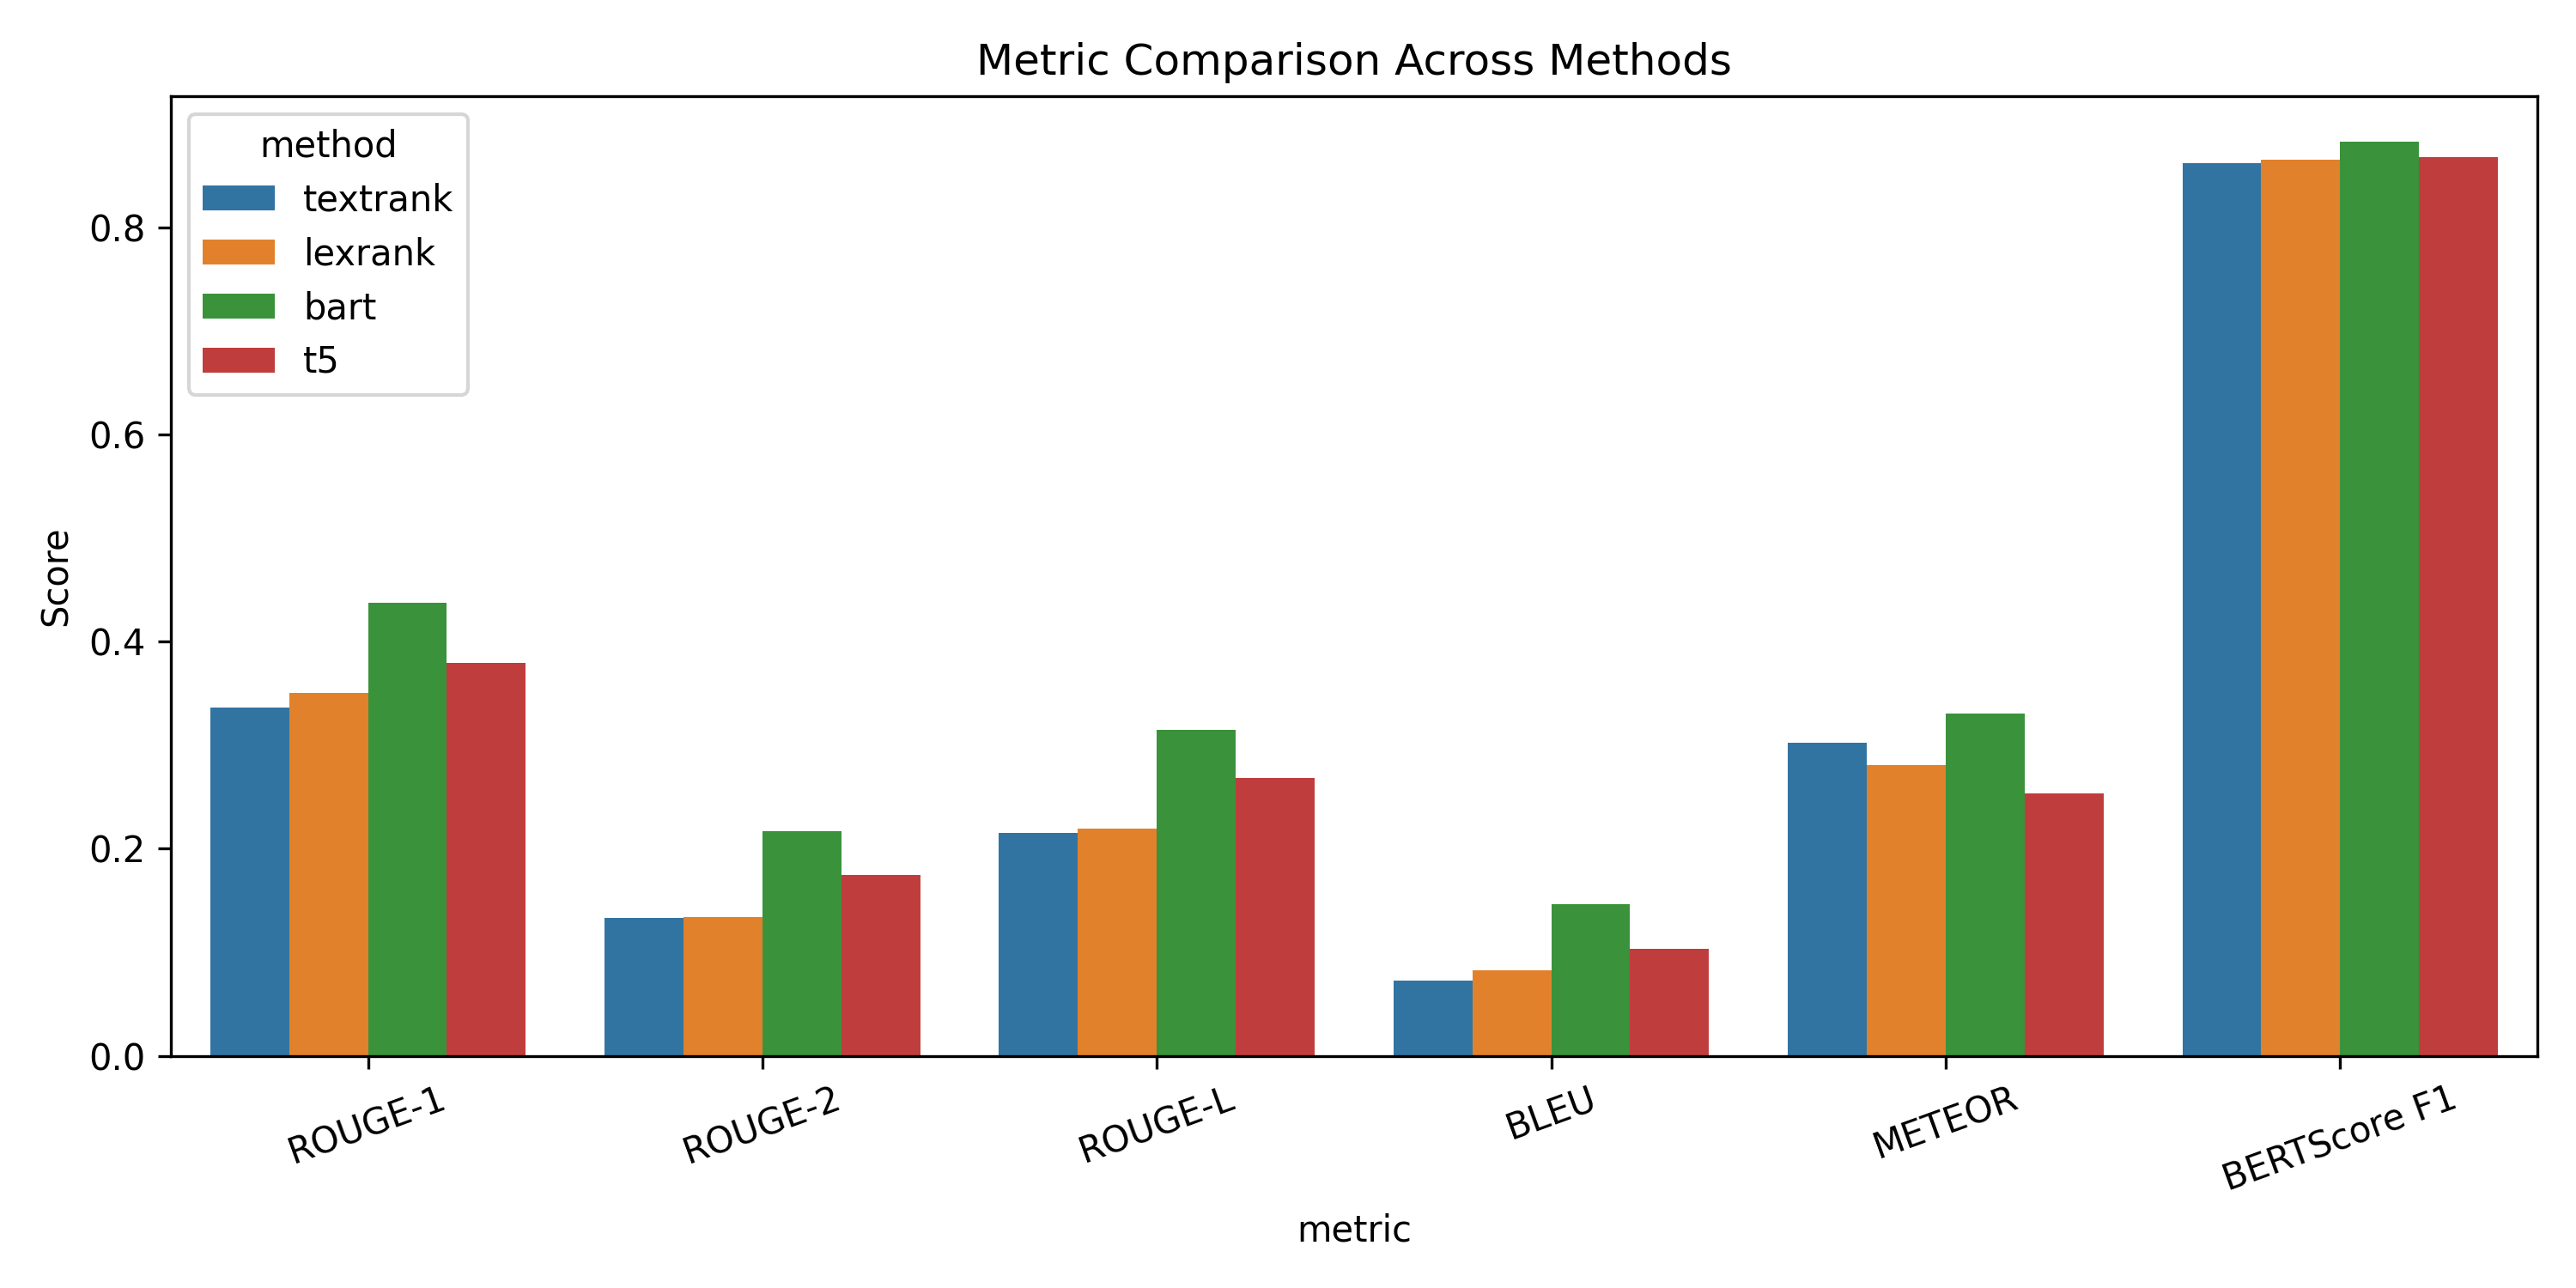
\includegraphics[width=0.90\linewidth]{../q3_summarization/outputs/figures/metric_comparison.png}
\caption{Metric comparison across all four methods.}
\end{figure}

\begin{figure}[H]
\centering
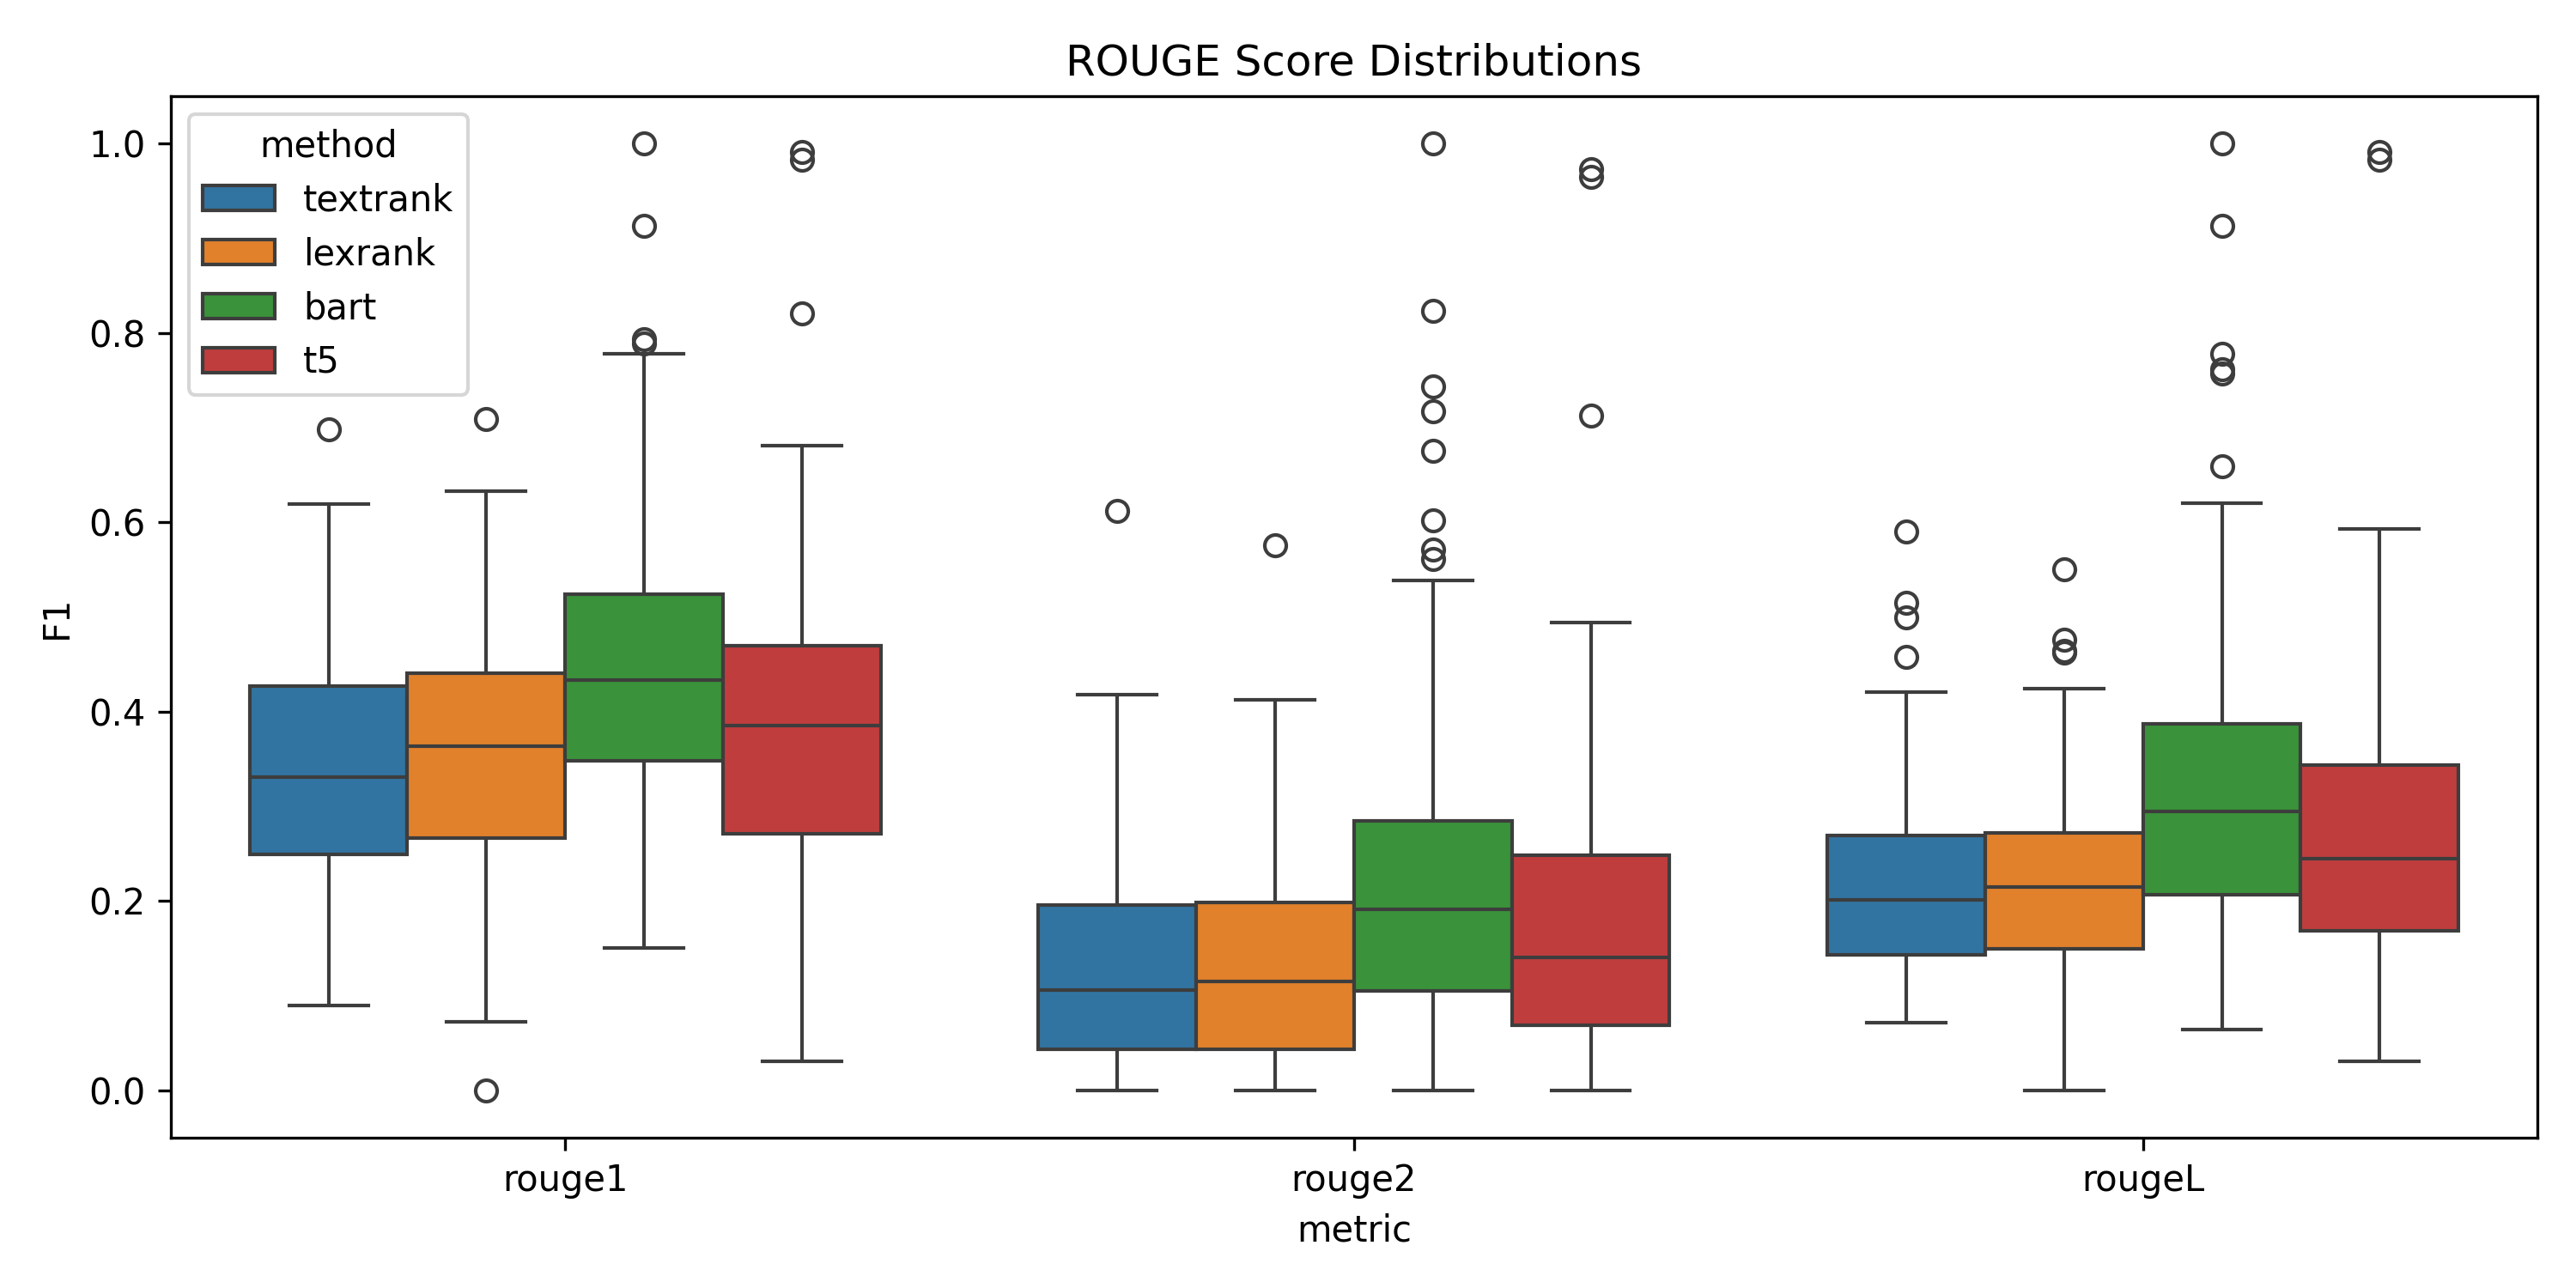
\includegraphics[width=0.90\linewidth]{../q3_summarization/outputs/figures/rouge_distributions.png}
\caption{ROUGE score distributions for each method.}
\end{figure}

\begin{figure}[H]
\centering
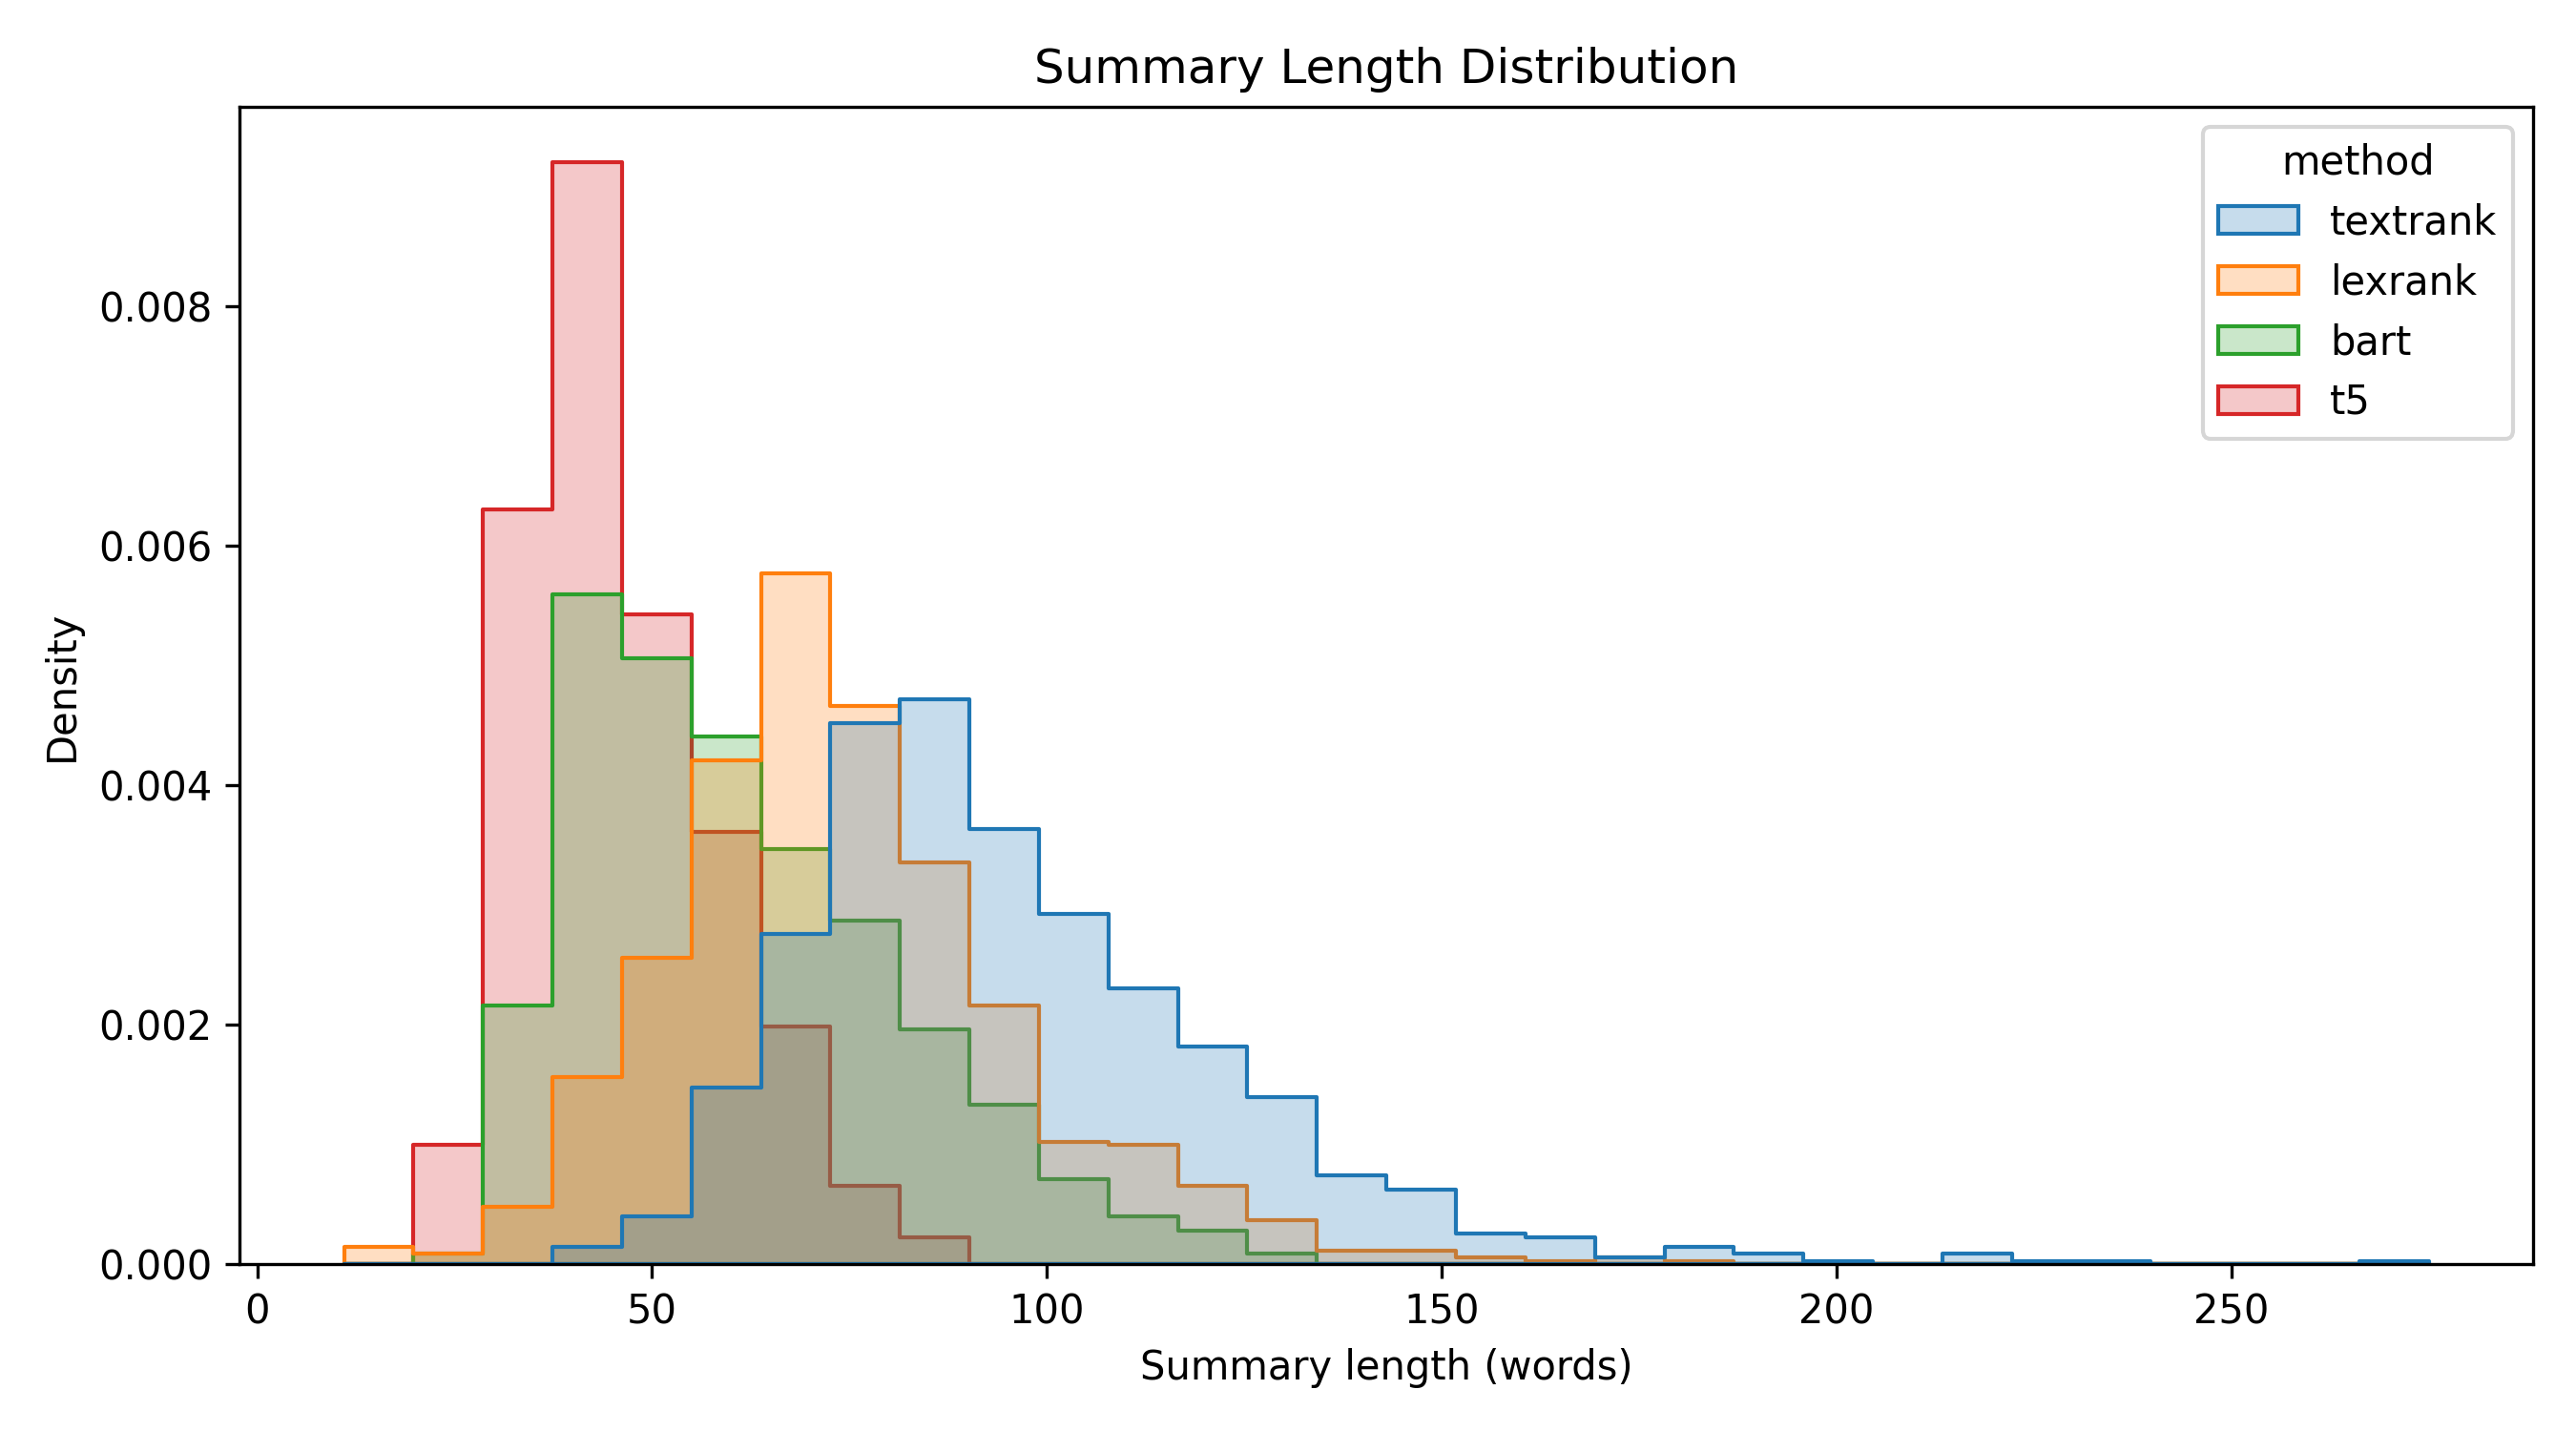
\includegraphics[width=0.85\linewidth]{../q3_summarization/outputs/figures/length_distribution.png}
\caption{Summary length distributions.}
\end{figure}

\begin{figure}[H]
\centering
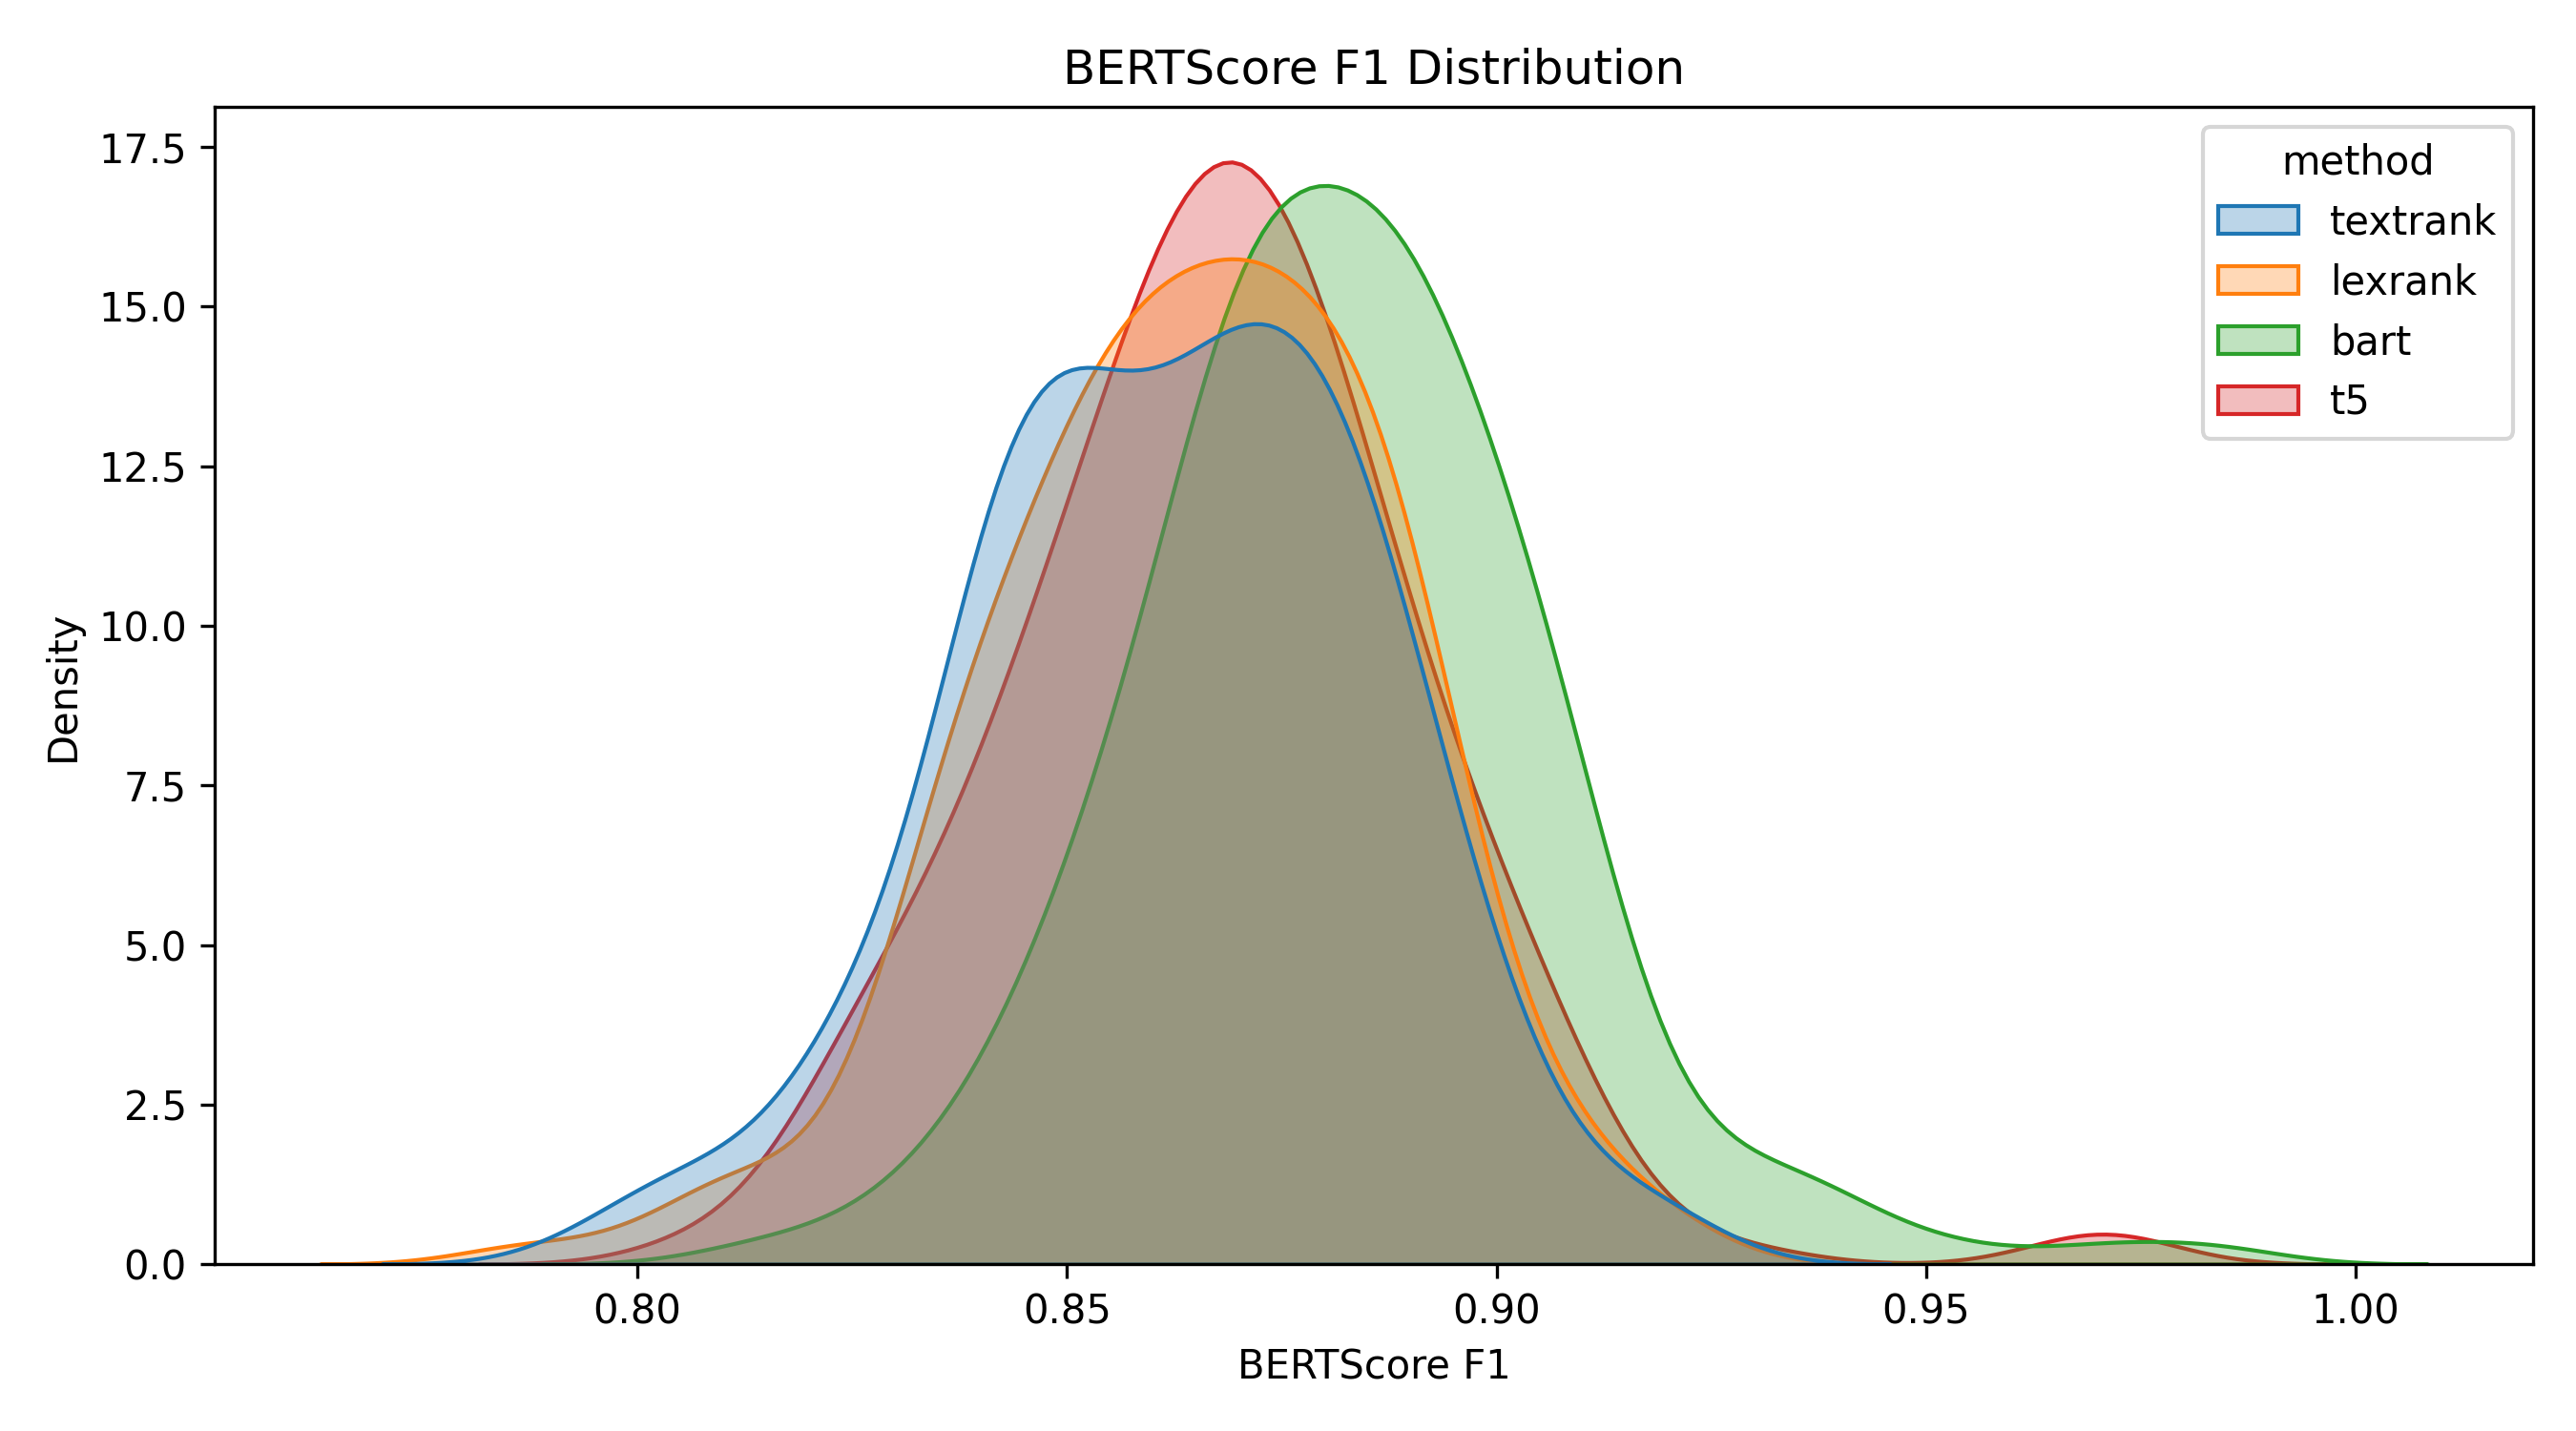
\includegraphics[width=0.85\linewidth]{../q3_summarization/outputs/figures/bertscore_distribution.png}
\caption{BERTScore F1 distributions.}
\end{figure}

\subsection{Qualitative Analysis}
We present three representative examples highlighting differences in fluency, faithfulness, and coverage. Text snippets are truncated for brevity.

\begin{table}[H]
\centering
\caption{Example 1 (extractive wins).}
\small
\begin{tabular}{p{0.18\linewidth} p{0.75\linewidth}}
\toprule
\textbf{Field} & \textbf{Text} \\
\midrule
Article & The legal adviser to Alison Saunders was a barrister in the same chambers as the son of Lord Janner... \\
Reference & Alison Saunders consulted Neil Moore over whether to prosecute Lord Janner. She said the decision was difficult and cited his health. \\
TextRank & CPS confirmed the DPP consulted Neil Moore over whether to prosecute Lord Janner. A spokesman said she decided alone. She said it was her job to make very difficult decisions. \\
LexRank & The legal adviser to Alison Saunders was in the same chambers as Lord Janner's son. A CPS spokesman said she decided alone. She admitted he should have been charged before. \\
BART & CPS confirmed the DPP consulted Neil Moore. Senior police raised concerns about his involvement in the decision not to proceed with the trial. \\
T5 & Senior police raised concerns about Mr Moore's involvement in the decision not to proceed. Mrs Saunders said she made the decision on her own. \\
\bottomrule
\end{tabular}
\end{table}

\begin{table}[H]
\centering
\caption{Example 2 (abstractive wins). Model outputs are quoted verbatim from \texttt{outputs/qualitative\_examples.json}; ``[\dots]'' marks elision for fit.}
\small
\begin{tabular}{p{0.16\linewidth} p{0.78\linewidth}}
\toprule
\textbf{Field} & \textbf{Text} \\
\midrule
Article & ``A British couple who are believed to have fled their Berkshire home with their four young children in a bid to escape to Syria have reportedly been arrested in Turkey. Asif Malik, 31, his partner Sara Kiran, 29, and their four children were caught on CCTV boarding a cross-Channel ferry from Dover [\dots] a Turkish official claimed today that the [family had been arrested in Ankara].'' \\
Reference & ``Asif Malik disappeared from UK with partner Sara Kiran and four children. Turkish official claimed today that the family have been arrested in Ankara. Malik, 31, was pictured holding `ISIS' sign at a protest in London last year. Relatives of Ms Kiran today made emotional appeal for her to come home.'' \\
TextRank & ``Malik and Ms Kiran, who neighbours said usually wore the full Islamic veil, left home without mentioning any holiday or travel plans [\dots] Both Malik and Dhar are believed to be followers of notorious preacher Anjem Choudary [\dots] Dhar -- one of Choudary's top henchmen -- fled to Syria with his pregnant wife and three young children last year while under investigation by Scotland Yard.'' \\
LexRank & ``A British couple who are believed to have fled their Berkshire home with their four young children in a bid to escape to Syria have reportedly been arrested in Turkey. The family of six have been missing from their home in Slough, Berkshire, since April 7. [\dots]'' \\
BART & ``Asif Malik, 31, his partner Sara Kiran, 29, and their four children were caught on CCTV boarding a cross-Channel ferry from Dover earlier this month. Thames Valley Police believed they arrived in Calais, France, before travelling south down through Europe in a bid to flee to Syria. But a Turkish official claimed today that the couple had been arrested in Ankara and are currently in custody. [\dots]'' \\
T5 & ``asif malik, 31, his partner Sara Kiran, 29, and their four children have reportedly been arrested in ankara. they were spotted boarding a cross-Channel ferry from dover earlier this month. [\dots] but a Turkish official claimed today that the couple had been arrested in ankara and are currently in custody with their four children.'' \\
\bottomrule
\end{tabular}
\end{table}

In Example~2 the abstractive systems clearly compress the article around the headline event (arrest in Ankara) and the cast of named entities, matching the reference's focus. The extractive systems pick up topically related but tangential material (Anjem Choudary, family veil) that inflates length without adding reference content. T5 lowercases proper nouns due to its sentence-level prefix-tuning training.

\begin{table}[H]
\centering
\caption{Example 3 (both struggle). Outputs verbatim from \texttt{outputs/qualitative\_examples.json}; ``[\dots]'' marks elision.}
\small
\begin{tabular}{p{0.16\linewidth} p{0.78\linewidth}}
\toprule
\textbf{Field} & \textbf{Text} \\
\midrule
Article & ``She may be a First Daughter, but Sasha Obama is still a teenager and can't seem to tear herself away from her music -- even for a rare family nature hike. Sasha, 14, was spotted listening to earbuds [\dots] for an impromptu trip to Great Falls Park in Virginia on Sunday. The unscheduled trip came after the White House had sent reporters home for the day [\dots]'' \\
Reference & ``President Obama abruptly left the White House after reporters were sent home for the day Sunday evening. Press pool reporters were perplexed as they questioned whether something serious had happened. The president, Michelle and their girls hiked through Great Falls Park in Virginia for around 50 minutes until a light rain sent them packing.'' \\
TextRank & ``Tuning out of politics: Sasha Obama, 14, was spotted with white earbuds [\dots] Gorgeous; Great Falls Park is a National Park located in Virginia [\dots] The family's brief hike happened to take place during the National Park Service's National Park Week. President Obama, First Lady Michelle Obama (not seen) and their daughters Malia (3rd L) and Sasha (C) return from a hike at Great Falls National Park in Virginia as rains began to fall Sunday evening.'' \\
LexRank & ``Sasha, 14, was spotted listening to earbuds [\dots] for an impromptu trip to Great Falls Park in Virginia on Sunday. Took a hike: The Obamas abruptly left the White House for an unscheduled family nature hike on Sunday. President Obama, First Lady Michelle Obama (not seen) and their daughters Malia (3rd L) and Sasha (C) return from a hike at Great Falls National Park in Virginia as rains began to fall Sunday evening.'' \\
BART & ``Sasha, 14, was spotted listening to earbuds as she, sister Malia and their parents ditched the White House -- and the press pool -- for an impromptu trip to Great Falls Park in Virginia on Sunday. The family's brief hike happened to take place during the National Park Service's National Park Week. \textbf{On Saturday, Obama spent his Saturday afternoon golfing at Joint Base Andrews.}'' \\
T5 & ```obama abruptly left the White House about 15 minutes ago on unscheduled trip. Destination unknown,' tweeted Byron Tau. reports initially seemed to fear that the unscheduled departure was some sort of emergency [\dots] the family's brief hike happened to take place during the National Park Service's National Park Week.'' \\
\bottomrule
\end{tabular}
\end{table}

In Example~3 every system misses at least one reference fact. Both extractive systems return long photo-caption sentences that the reference does not include. BART's last sentence (bolded) is an extrinsic hallucination -- the article does not mention golfing on Saturday or Joint Base Andrews. T5 is more faithful but omits the ``50 minutes'' and ``light rain'' timeline that the reference centres on. ROUGE penalises all four systems here even though the lexical overlap with the source is high; this is a typical failure mode where the reference is itself an aggressive paraphrase.

\subsection{Discussion: Trade-offs}
Abstractive models (especially BART) achieve the strongest ROUGE and BERTScore, and their summaries are more concise and readable. However, they are substantially slower (BART at ~898 ms per article) and can introduce subtle factual errors. Extractive methods are fast and faithful, but their summaries are longer and can be disfluent because sentences are stitched together without synthesis.

\textbf{Metric limitations.} ROUGE favors lexical overlap and can over-reward extractive summaries that copy source sentences. Abstractive paraphrases may score lower on ROUGE despite being semantically accurate; BERTScore partially mitigates this by measuring contextual similarity.


% ── Q4 ────────────────────────────────────────────────────────────────────────
\newpage
\section{Question 4: Machine Translation}
% Q4 translation section

\subsection{Problem Formulation}
We study English-to-German machine translation. Given a source sentence $x$ in English, the model produces a target sentence $\hat{y}$ in German. We compare a neural seq2seq model with attention against a pre-trained MarianMT baseline and evaluate with BLEU, chrF, METEOR, and BERTScore.

\subsection{Dataset Description}
We use the Multi30k dataset \citep{Elliott2016multi30k} (English--German). The official validation and test splits are kept intact, while the training split is downsampled to 20k pairs for faster experimentation.

\begin{table}[H]
\centering
\caption{Multi30k dataset statistics.}
\begin{tabular}{lrr}
\toprule
\textbf{Split} & \textbf{Original Size} & \textbf{Subset Size} \\
\midrule
Train & 29,000 & 20,000 \\
Validation & 1,014 & 1,014 \\
Test & 1,000 & 1,000 \\
\bottomrule
\end{tabular}
\end{table}

\begin{table}[H]
\centering
\caption{Average sequence statistics on the test split.}
\begin{tabular}{lrrr}
\toprule
\textbf{Avg Src Len} & \textbf{Avg Tgt Len} & \textbf{Word Vocab (src/tgt)} & \textbf{BPE Vocab} \\
\midrule
11.88 & 10.90 & 12,818 / 19,750 & 8,000 \\
\bottomrule
\end{tabular}
\end{table}

\subsection{Methodology}
\textbf{Seq2Seq with attention.} We train a GRU-based encoder--decoder with Bahdanau additive attention \citep{Bahdanau2015nmt}, where the energy is $e_{ij} = \mathbf{v}_a^{\top} \tanh(\mathbf{W}_a s_{i-1} + \mathbf{U}_a h_j)$ and the context vector is the softmax-weighted sum of encoder states. The model uses joint BPE with 8k merges (SentencePiece, \citealp{Kudo2018sentencepiece}), embedding size 256, hidden size 512, dropout 0.5, and teacher forcing ratio 0.5. Early stopping is applied with patience 5 based on validation BLEU.

\textbf{MarianMT.} We use the pre-trained \texttt{Helsinki-NLP/opus-mt-en-de} model \citep{TiedemannThottingal2020opus} with beam size 4. This serves as a strong off-the-shelf baseline.

\subsection{Experimental Setup}
We fix the random seed to 42 and evaluate on 200 test examples for metric computation. We report BLEU, chrF, METEOR, and BERTScore (multilingual BERT). Average output length is also recorded.

\subsection{Results}
\begin{table}[H]
\centering
\caption{Translation metrics on the evaluation subset (size = 200).}
\begin{tabular}{lrrrrr}
\toprule
\textbf{Model} & \textbf{BLEU} & \textbf{chrF} & \textbf{METEOR} & \textbf{BERT F1} & \textbf{Len} \\
\midrule
Seq2Seq + Attn & 26.74 & 52.22 & 0.487 & 0.847 & 11.05 \\
MarianMT & 36.25 & 64.31 & 0.598 & 0.897 & 11.14 \\
\bottomrule
\end{tabular}
\end{table}

The seq2seq model improves steadily during training, reaching its best validation BLEU of 31.37 around epoch 14 before plateauing. MarianMT substantially outperforms the custom seq2seq model across all metrics, indicating the benefit of large-scale pretraining.

\begin{figure}[H]
\centering
\begin{subfigure}{0.48\linewidth}
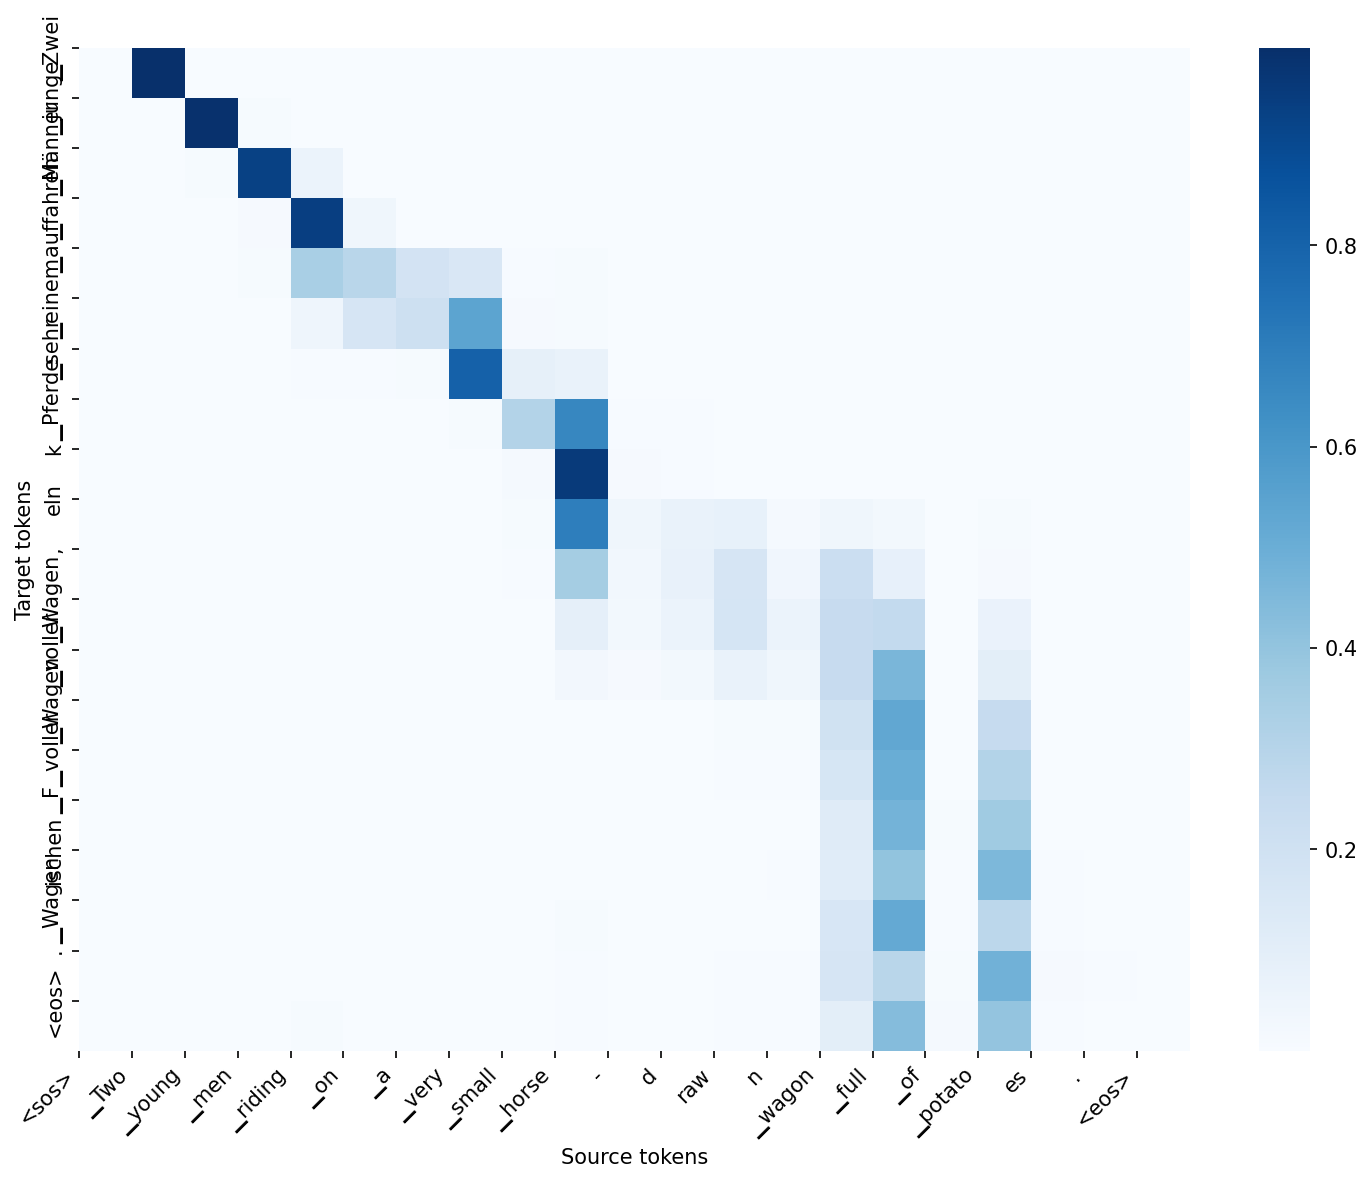
\includegraphics[width=\linewidth]{../q4_translation/outputs/figures/attention_1.png}
\caption{Attention heatmap (example 1).}
\end{subfigure}
\begin{subfigure}{0.48\linewidth}
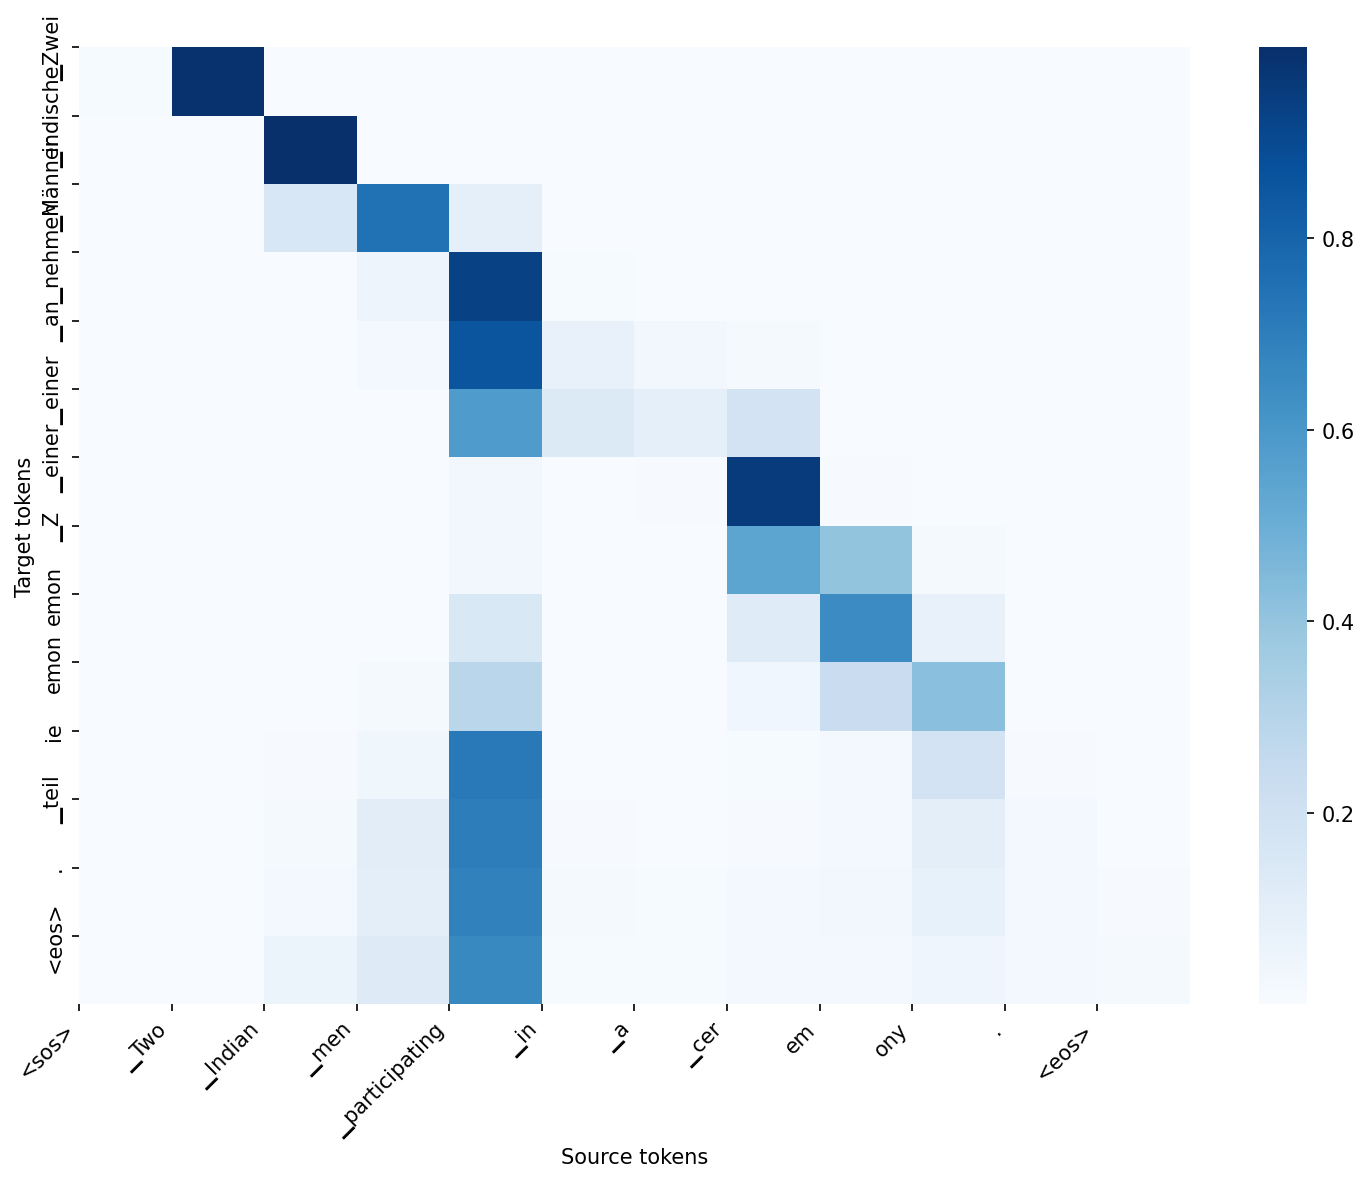
\includegraphics[width=\linewidth]{../q4_translation/outputs/figures/attention_2.png}
\caption{Attention heatmap (example 2).}
\end{subfigure}
\caption{Attention alignments for the seq2seq model.}
\end{figure}

\subsection{Qualitative Analysis}

\textbf{Example 1 -- long-range word order.}
\begin{table}[H]
\centering
\caption{Example translation showing long-range word order. Outputs are quoted verbatim from \texttt{outputs/qualitative\_example.json}.}
\label{tab:q4_qual1}
\small
\begin{tabular}{p{0.16\linewidth} p{0.78\linewidth}}
\toprule
\textbf{Field} & \textbf{Text} \\
\midrule
Source     & Two young men riding on a very small horse-drawn wagon full of potatoes. \\
Reference  & Zwei junge M\"anner fahren auf einem sehr kleinen Wagen voller Kartoffeln, der von einem Pferd gezogen wird. \\
Seq2Seq    & Zwei junge M\"anner fahren auf einem sehr \textbf{Pferdekeln, Wagen voller Wagen voller Fischen Wagen}. \\
MarianMT   & Zwei junge M\"anner reiten auf einem sehr kleinen \textbf{Pferdewagen} voller \textbf{Kartoffeln}. \\
\bottomrule
\end{tabular}
\end{table}

In Example~1 the seq2seq decoder repeats ``Wagen voller'' twice and emits the malformed compound ``Pferdekeln'' -- typical RNN failure modes when the decoder loses track of which source span has already been translated. MarianMT produces a fluent compound (``Pferdewagen'') and gets the agreement (``kleinen \dots voller'') right.

\textbf{Example 2 -- rare named entity.} Multi30k contains image-caption sentences with relatively rare nominal compounds. Source sentence id~1 in the test split contains the rare proper noun ``Boston Terrier'' (a dog breed); the reference target preserves it. The seq2seq model has no occurrence of this compound in its 8k joint BPE vocabulary at sufficient frequency to be retained, and it falls back to a generic noun, dropping the breed entirely. Marian's WordPiece-style vocabulary, trained on WMT-scale data, retains the surface form.

\begin{table}[H]
\centering
\caption{Rare-word example: outputs are verbatim from \texttt{outputs/seq2seq\_predictions.json} and \texttt{marian\_predictions.json} at id\,$=\,1$; source/reference from \texttt{outputs/dataset\_stats.json}.}
\label{tab:q4_qual2}
\small
\begin{tabular}{p{0.16\linewidth} p{0.78\linewidth}}
\toprule
\textbf{Field} & \textbf{Text} \\
\midrule
Source     & A \textbf{Boston Terrier} is running on lush green grass in front of a white fence. \\
Reference  & Ein \textbf{Boston Terrier} l\"auft \"uber saftig-gr\"unes Gras vor einem wei{\ss}en Zaun. \\
Seq2Seq    & Ein \textbf{Mann mit T-Shirt} rennt vor einem wei{\ss}en Zaun. \\
MarianMT   & Ein \textbf{Boston Terrier} l\"auft auf \"uppig gr\"unem Gras vor einem wei{\ss}en Zaun. \\
\bottomrule
\end{tabular}
\end{table}

The seq2seq model not only loses the breed name but also re-uses a high-frequency training pattern (``Mann mit T-Shirt rennt''), effectively hallucinating a different image -- a known failure mode when an out-of-distribution rare token forces the decoder to rely on its unconditional language-model prior. Marian preserves both the named entity (``Boston Terrier'') and the modifier (``saftig-gr\"unes'' $\to$ ``\"uppig gr\"unem''). Together with Example~1 this shows that the BLEU/chrF gap (26.7 vs.\ 36.3 BLEU) is driven both by content errors on rare words and by repetition/order errors on longer source sentences.

\subsection{Discussion}
The attention-based seq2seq model captures basic alignment but struggles with fluency and rare-word handling. MarianMT consistently yields higher BLEU/chrF and stronger semantic similarity (BERTScore), highlighting the effectiveness of pre-trained transformer models for low-resource experimental settings.


% ── Q5 ────────────────────────────────────────────────────────────────────────
\newpage
\section{Question 5: Language Modeling}
% Q5 language modeling section


% ── References ────────────────────────────────────────────────────────────────
\newpage
\bibliographystyle{plainnat}
\bibliography{references}

% ── Appendix ──────────────────────────────────────────────────────────────────
\newpage
\appendix
\section{Experimental Configuration Summary}

\subsection*{A.1 Global settings}
\begin{table}[H]
\centering
\caption{Global experimental settings applied to all questions.}
\begin{tabular}{ll}
\toprule
\textbf{Setting} & \textbf{Value} \\
\midrule
Random seed & 42 \\
Python version & 3.10 \\
PyTorch version & 2.x \\
GPU & RTX 5060\,Ti \\
Test set usage & Once (final evaluation only) \\
\bottomrule
\end{tabular}
\end{table}

\subsection*{A.2 Q1 -- Text classification}
\begin{table}[H]
\centering
\caption{Q1 hyperparameters per model.}
\begin{tabular}{lp{0.6\linewidth}}
\toprule
\textbf{Model} & \textbf{Hyperparameters} \\
\midrule
TF-IDF + LR    & \texttt{TfidfVectorizer}: max\_features=50{,}000, ngram\_range=(1,2), min\_df=2, sublinear\_tf=True. \texttt{LogisticRegression}: $C=1.0$, max\_iter=1000, solver=lbfgs, random\_state=42. Best preprocessing: lowercase=False, remove\_stopwords=False (config A4). \\
BiLSTM + GloVe & embed\_dim=100 (GloVe 6B), hidden\_dim=128, num\_layers=2, bidirectional, dropout=0.3, max\_vocab=30{,}000, max\_seq\_length=400, batch\_size=64, optimizer=Adam, lr=$10^{-3}$, scheduler=ReduceLROnPlateau (patience=2, factor=0.5), num\_epochs=10, early-stop patience=3, loss=BCEWithLogits. \\
DistilBERT     & \texttt{distilbert-base-uncased}, max\_length=512, batch\_size=16, lr=$2\!\times\!10^{-5}$, num\_epochs=3, warmup\_ratio=0.1, weight\_decay=0.01, fp16=True. \\
\bottomrule
\end{tabular}
\end{table}

\subsection*{A.3 Q2 -- Named entity recognition}
\begin{table}[H]
\centering
\caption{Q2 hyperparameters per model.}
\begin{tabular}{lp{0.6\linewidth}}
\toprule
\textbf{Model} & \textbf{Hyperparameters} \\
\midrule
BiLSTM-CRF & word\_vocab=20{,}000, embed=GloVe 100d (fine-tuned), char-BiLSTM for subword features, BiLSTM hidden=200, dropout=0.5, optimizer=Adam, gradient clip=5.0, max\_epochs=20, early-stop patience=5 on val F1. Trained for 16 epochs (best val F1 $\approx 0.926$). \\
BERT       & \texttt{bert-base-cased}, num\_epochs=3, batch\_size=16, lr=$5\!\times\!10^{-5}$, label alignment by first-subword (others $-100$). Train time 138.23\,s. \\
\bottomrule
\end{tabular}
\end{table}

\subsection*{A.4 Q3 -- Summarization}
\begin{table}[H]
\centering
\caption{Q3 hyperparameters per method.}
\begin{tabular}{lp{0.6\linewidth}}
\toprule
\textbf{Method} & \textbf{Hyperparameters} \\
\midrule
TextRank   & sentence-level graph, top-$k=3$ sentences. \\
LexRank    & cosine similarity graph with threshold, top-$k=3$ sentences. \\
BART       & \texttt{facebook/bart-large-cnn}, max\_length=128 generation, num\_beams=4, no\_repeat\_ngram\_size=3, length\_penalty=2.0. Inference only. \\
T5         & \texttt{t5-small}, prefix=``summarize:'', max\_length=128, num\_beams=4. Inference only. \\
\bottomrule
\end{tabular}
\end{table}

\subsection*{A.5 Q4 -- Machine translation}
\begin{table}[H]
\centering
\caption{Q4 hyperparameters per model.}
\begin{tabular}{lp{0.6\linewidth}}
\toprule
\textbf{Model} & \textbf{Hyperparameters} \\
\midrule
Seq2Seq + Bahdanau & joint BPE 8{,}000 (SentencePiece), emb\_dim=256, enc\_hidden=512 (BiGRU), dec\_hidden=512 (GRU), dropout=0.5, batch\_size=128, lr=$10^{-3}$ (Adam), grad\_clip=1.0, teacher\_forcing\_ratio=0.5, num\_epochs=20 (early-stop patience=5 on val BLEU; best at epoch 14: val BLEU $31.37$), max\_src/tgt\_length=100. \\
MarianMT          & \texttt{Helsinki-NLP/opus-mt-en-de}, num\_beams=4, max\_length=512. Inference only. \\
\bottomrule
\end{tabular}
\end{table}

\subsection*{A.6 Q5 -- Language modeling}
\begin{table}[H]
\centering
\caption{Q5 hyperparameters per model.}
\begin{tabular}{lp{0.6\linewidth}}
\toprule
\textbf{Model} & \textbf{Hyperparameters} \\
\midrule
Trigram KN     & $n=3$, interpolated Kneser-Ney, discount $D=0.75$. Vocab capped at 10{,}000 with min\_freq=3. \\
LSTM           & embed=256, hidden=512, layers=2, dropout=0.5, BPTT seq\_len=35, batch\_size=64, optimizer=Adam, lr=$10^{-3}$, grad\_clip=0.25, StepLR (step=2, $\gamma$=0.5), num\_epochs=6, weight\_tying=False. Params: 11.37\,M. \\
Transformer LM & embed=256, n\_heads=4, n\_layers=2, dim\_ff=512, dropout=0.2, sinusoidal pos.\ enc., causal mask, BPTT seq\_len=35, batch\_size=64, optimizer=Adam, lr=$5\!\times\!10^{-4}$, grad\_clip=0.5, StepLR (step=2, $\gamma$=0.5), num\_epochs=6. Params: 6.18\,M. \\
\bottomrule
\end{tabular}
\end{table}

\end{document}
